\errorcontextlines=100
%\documentclass[final]{ltugboat}
\documentclass[twoside,twocolumn]{scrartcl}
%% $Id: doublepage2s2c.tex 97 2021-05-26 19:31:53Z herbert $

\documentclass[a4paper,11pt]{article}
\usepackage[color]{lapdf}
\textheight25.12cm
\textwidth18.92cm
\oddsidemargin-1.5cm
\evensidemargin-1.5cm
\topmargin-0.5cm
\topskip0cm
\headheight0cm
\headsep0cm
\parskip0.5cm
\parindent0cm
\unitlength1cm


\usepackage{blindtext,xcolor,marginnote}

\let\hvBlindtext\Blindtext
\def\Blindtext{\par\color{black!40}\hvBlindtext\par\normalcolor}
\makeatletter
\def\hvblindtext{\textcolor{black!40}{\blindtext@text}}
\makeatother
\usepackage{marginnote,showframe}
\setcounter{tocdepth}{2}

\begin{document}
\title{Examples for doublepage floats \newline with bind correction}
\author{Herbert Voß}
\maketitle

\tableofcontents


\onecolumn
\listoffigures

\newpage\null
\twocolumn
\section{Argument \texttt{doublePage}}
\subsection{Definition on an odd page}

\Blindtext\hvblindtext

\hvblindtext

\subsubsection{The default}


\begin{lstlisting}
\hvFloat[doublePage]%,capWidth=n,capPos=right]%
  {figure}%
  {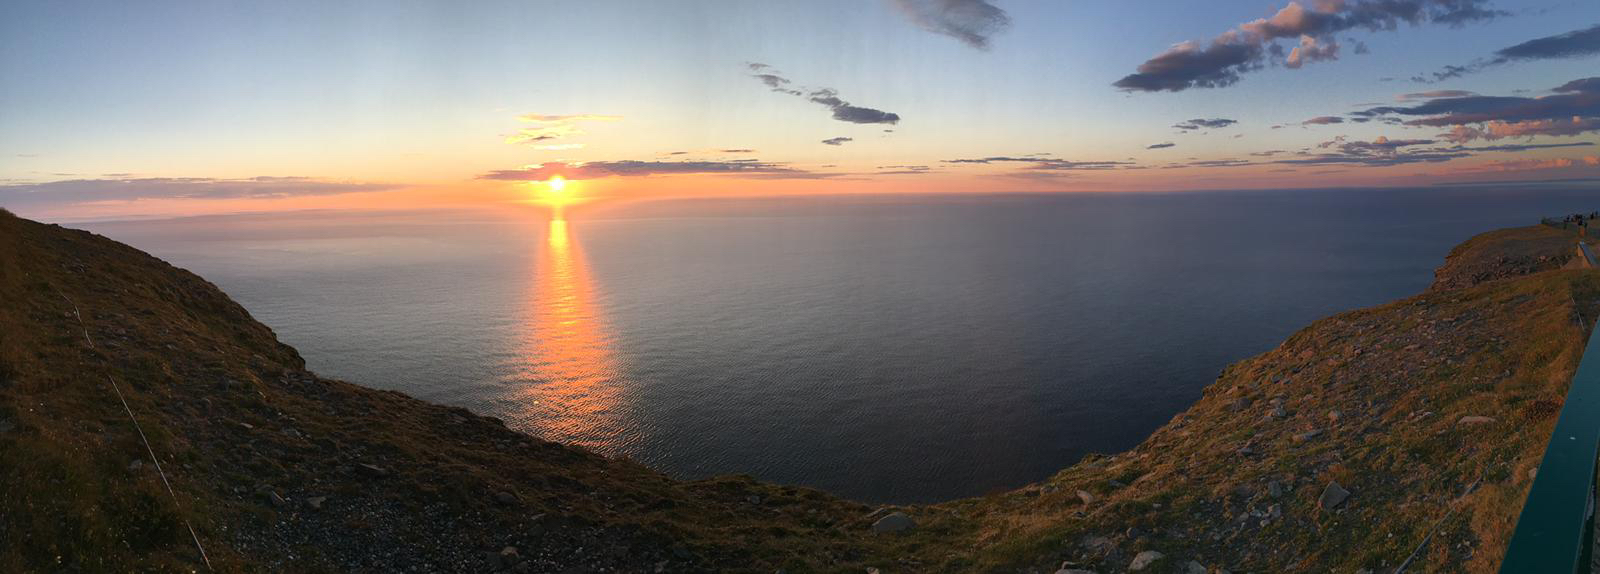
\includegraphics[width=2\textwidth]{images/sonne-meer}}%
  [A doublepage image with a caption on the right side of the right part.]%
  {A caption for a double-sided image that will be placed on the right side of the
   right-hand part of the illustration. The illustration begins on the left edge of 
   the paper. A short form is used for the LOF. 
   The parameter is \texttt{doublePage}}%
  {fig:doublePage0}
\end{lstlisting}


\marginnote{Fig. \ref{fig:doublePage0}}
\hvFloat[doublePage]%,capWidth=n,capPos=right]%
  {figure}%
  {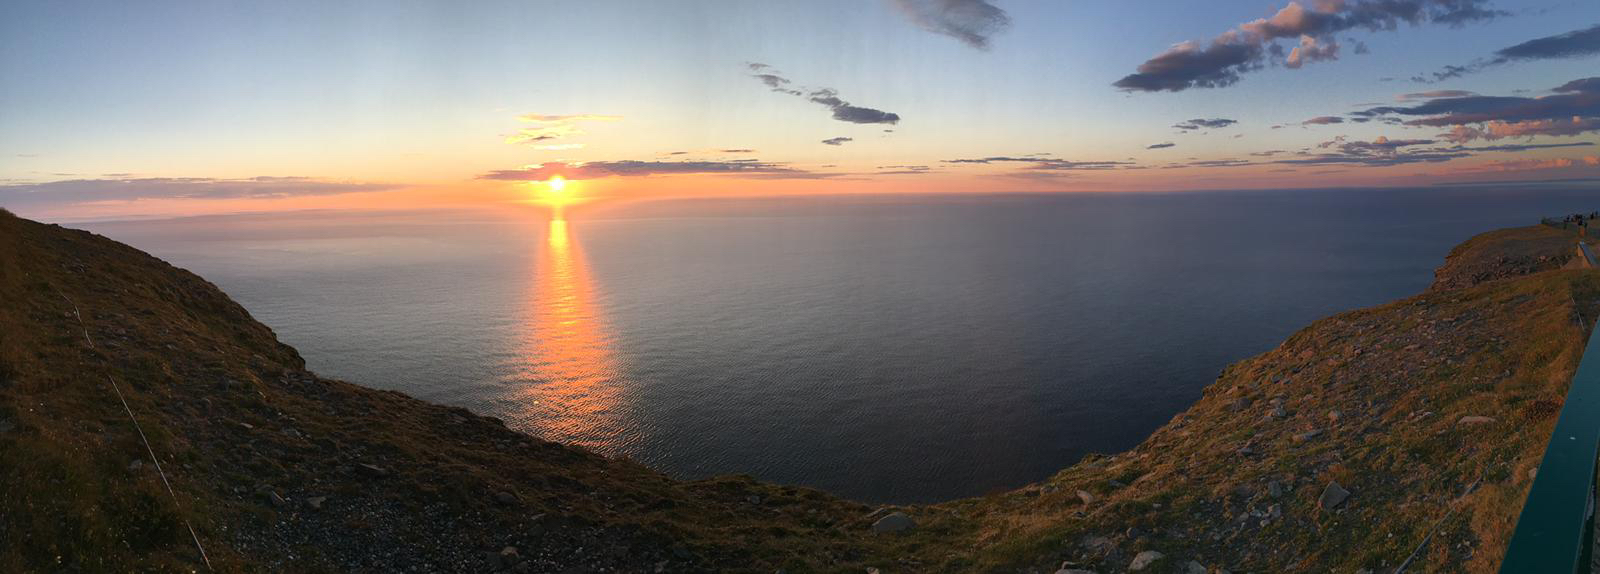
\includegraphics[width=2\textwidth]{images/sonne-meer}}%
  [A doublepage image with a caption on the right side of the right part.]%
  {A caption for a double-sided image that will be placed on the right side of the
   right-hand part of the illustration. The illustration begins on the left edge of 
   the paper. A short form is used for the LOF. 
   The parameter is \texttt{doublePage}}%
  {fig:doublePage0}

\Blindtext

\Blindtext

\Blindtext

\hvblindtext

\subsubsection{\texttt{bindCorr=1cm}}

\begin{lstlisting}
\hvFloat[doublePage,capWidth=n,capPos=right,bindCorr=1cm]%
  {figure}%
  {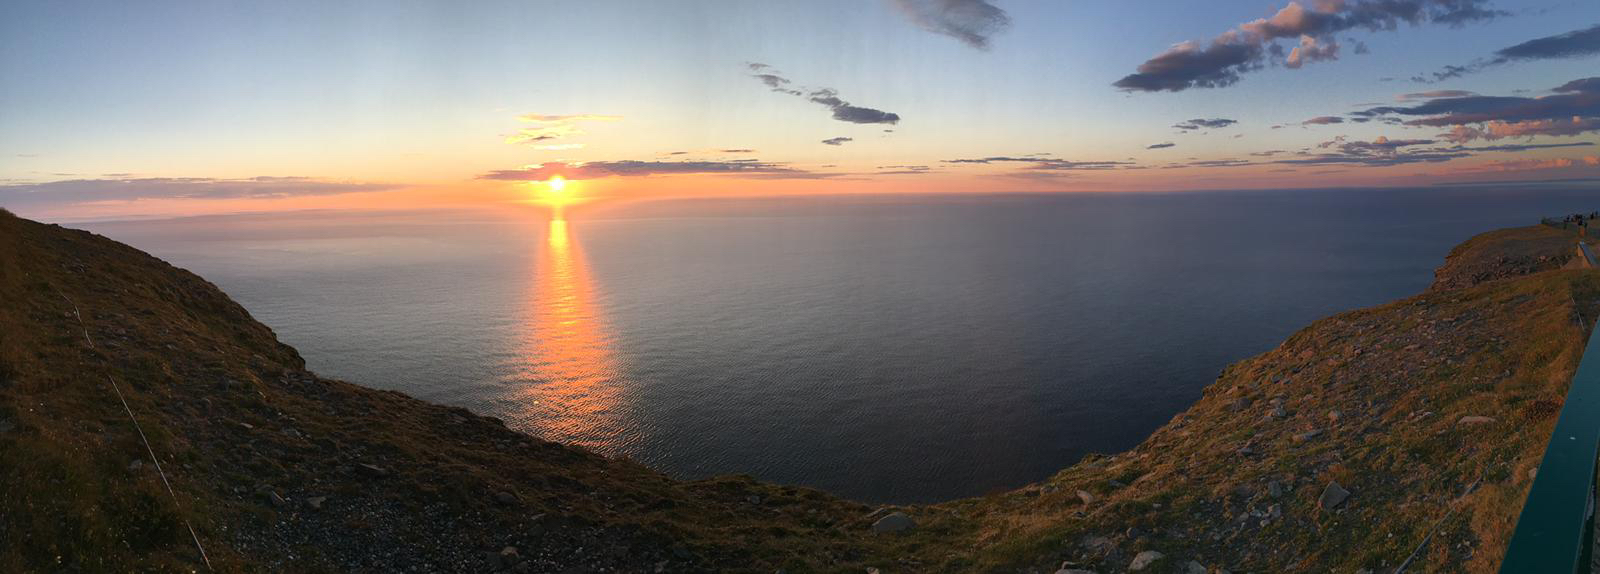
\includegraphics[width=2\textwidth]{images/sonne-meer}}%
  [A doublepage image with a caption on the right side of the right part.]%
  {A caption for a double-sided image that will be placed on the right side of the
   right-hand part of the illustration. The illustration begins on the left edge of 
   the paper. A short form is used for the LOF. 
   The parameter is \texttt{doublePage}}%
  {fig:doublePage1}
\end{lstlisting}

\marginnote{Fig. \ref{fig:doublePage1}}
\hvFloat[doublePage,capWidth=n,capPos=right,bindCorr=1cm]%
  {figure}%
  {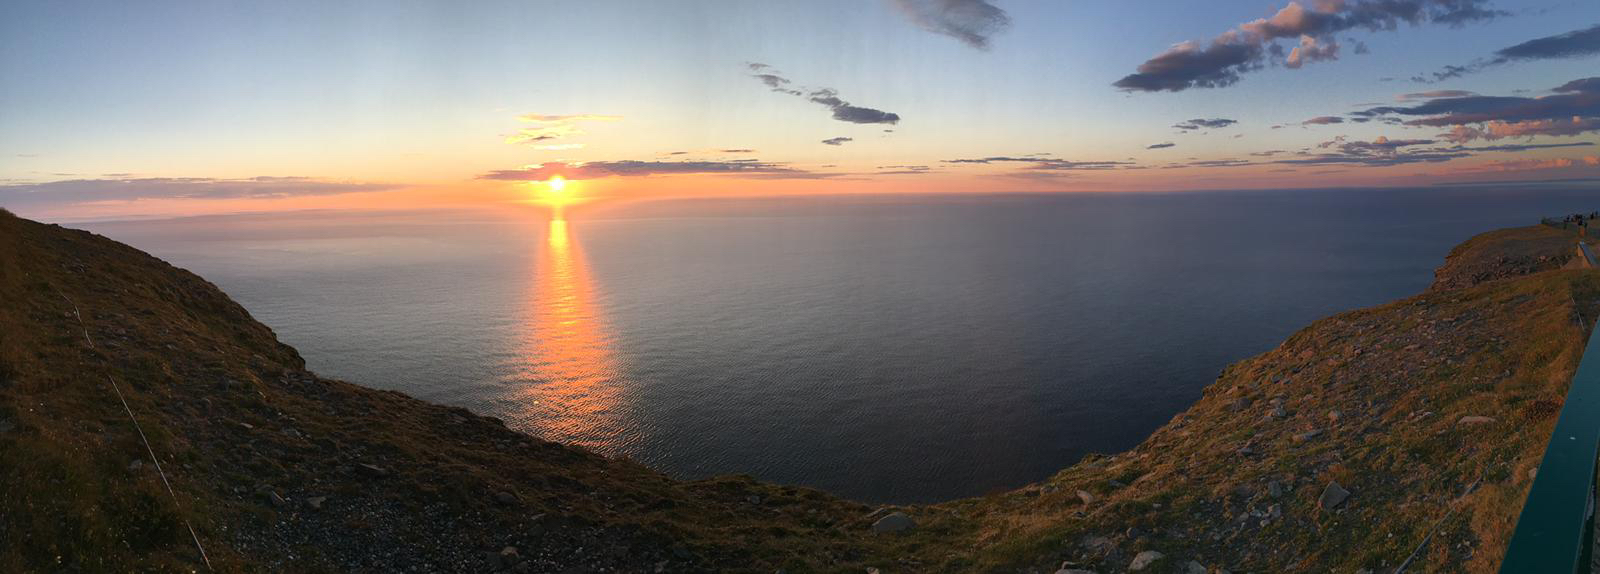
\includegraphics[width=2\textwidth]{images/sonne-meer}}%
  [A doublepage image with a caption on the right side of the right part.]%
  {A caption for a double-sided image that will be placed on the right side of the
   right-hand part of the illustration. The illustration begins on the left edge of 
   the paper. A short form is used for the LOF. 
   The parameter is \texttt{doublePage}}%
  {fig:doublePage1}

\hvblindtext

\Blindtext

\Blindtext

\Blindtext

\hvblindtext

\subsubsection{\texttt{bindCorr=3mm}}
\begin{lstlisting}
\hvFloat[doublePage,capWidth=n,capPos=right,bindCorr=3mm]%
  {figure}%
  {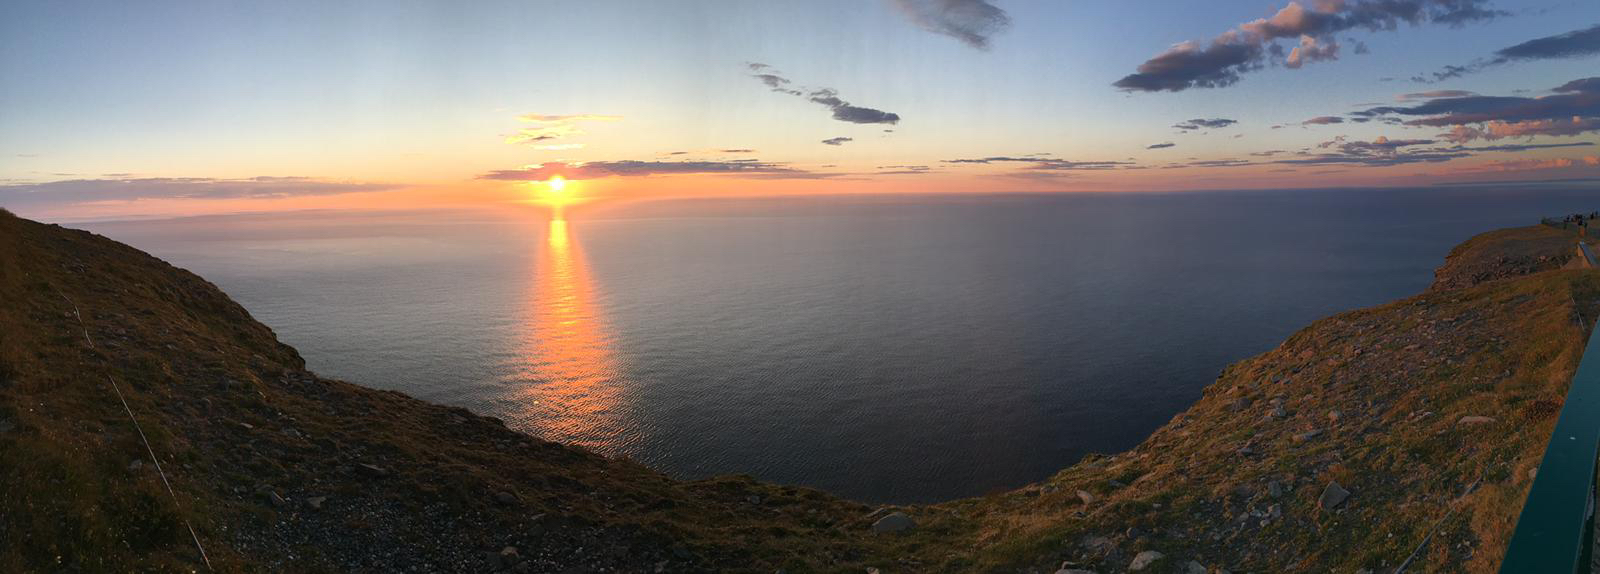
\includegraphics[width=2\textwidth]{images/sonne-meer}}%
  [A doublepage image with a caption on the right side of the right part.]%
  {A caption for a double-sided image that will be placed on the right side of the
   right-hand part of the illustration. The illustration begins on the left edge of 
   the paper. A short form is used for the LOF. 
   The parameter is \texttt{doublePage}}%
  {fig:doublePage2}
\end{lstlisting}

\marginnote{Fig. \ref{fig:doublePage2}}
\hvFloat[doublePage,capWidth=n,capPos=right,bindCorr=3mm]%
  {figure}%
  {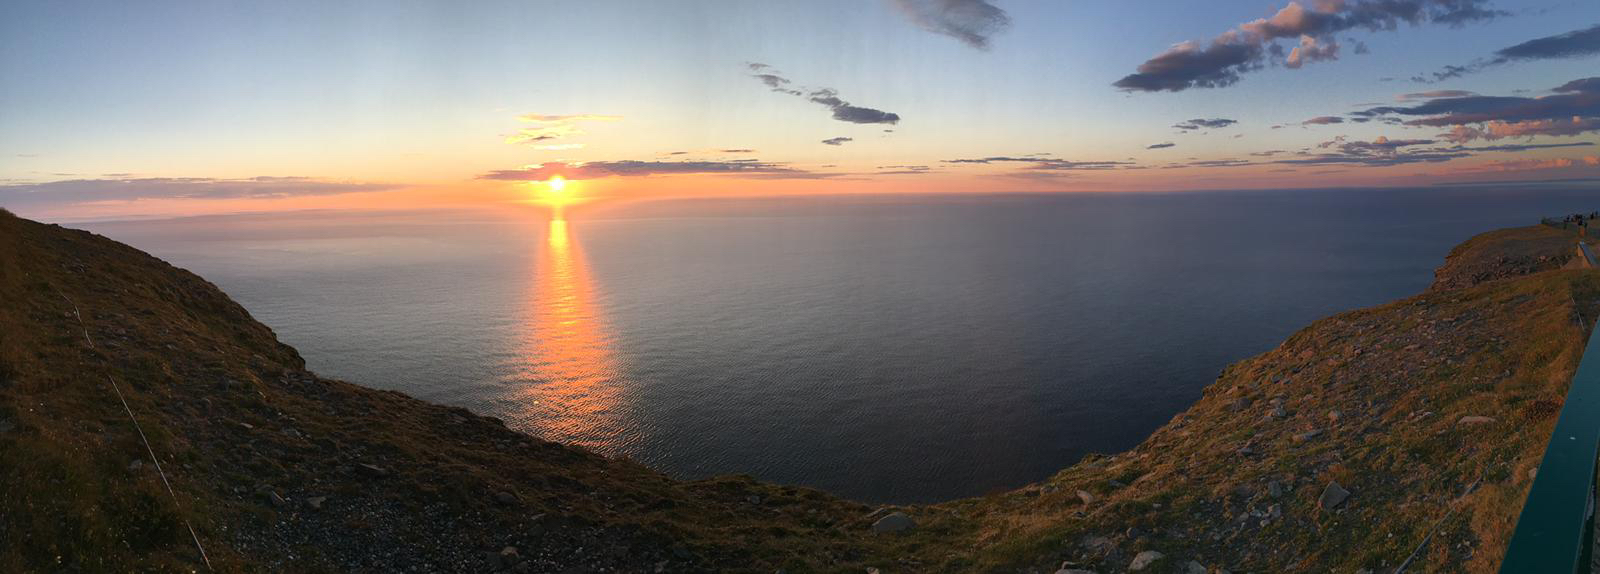
\includegraphics[width=2\textwidth]{images/sonne-meer}}%
  [A doublepage image with a caption on the right side of the right part.]%
  {A caption for a double-sided image that will be placed on the right side of the
   right-hand part of the illustration. The illustration begins on the left edge of 
   the paper. A short form is used for the LOF. 
   The parameter is \texttt{doublePage}}%
  {fig:doublePage2}


\Blindtext

\Blindtext

\Blindtext

\hvblindtext

\subsubsection{\texttt{bindCorr=<inside textwidth>}}

\begin{lstlisting}
\hvFloat[doublePage,capWidth=n,bindCorr=\the\dimexpr1in+\oddsidemargin]%
  {figure}%
  {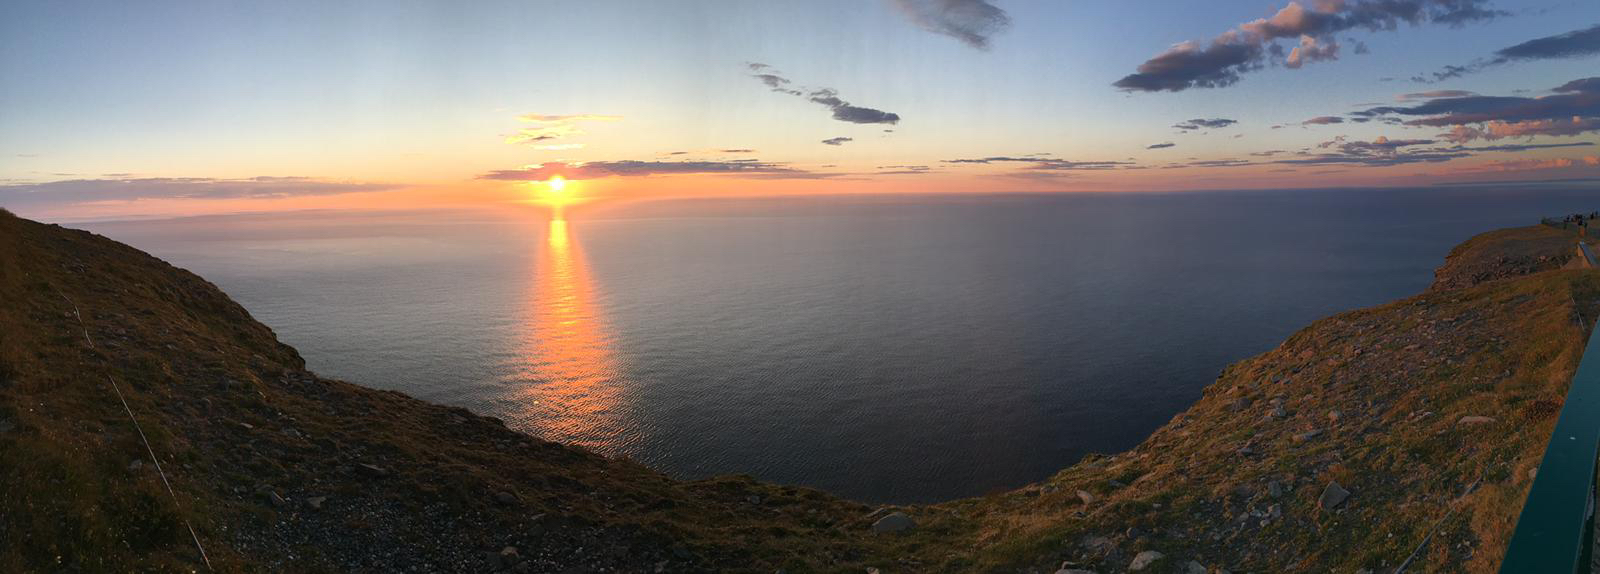
\includegraphics[width=2\textwidth]{images/sonne-meer}}%
  [A doublepage image with a caption on the right side of the right part.]%
  {A caption for a double-sided image that will be placed on the right side of the
   right-hand part of the illustration. The illustration begins on the left edge of 
   the paper. A short form is used for the LOF. 
   The parameter is \texttt{doublePage}}%
  {fig:doublePage3}
\end{lstlisting}

\marginnote{Fig. \ref{fig:doublePage3}}
\hvFloat[doublePage,capWidth=n,bindCorr=\the\dimexpr1in+\oddsidemargin]%
  {figure}%
  {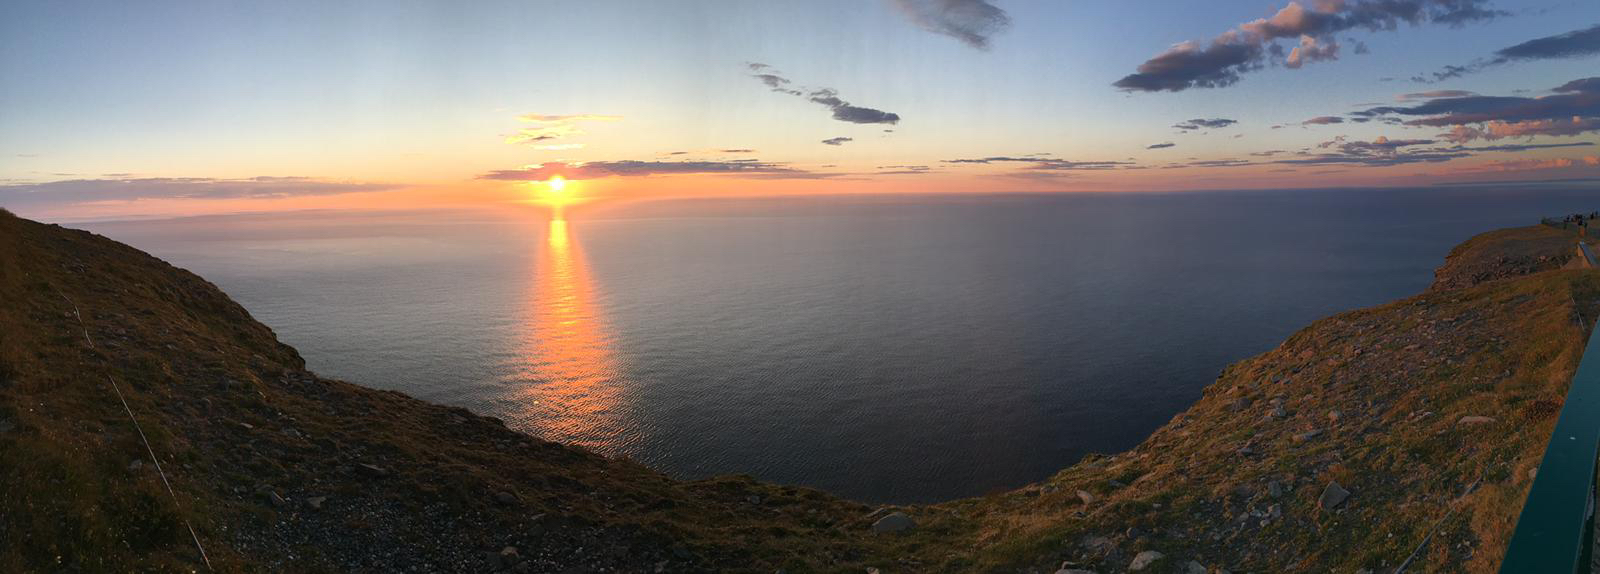
\includegraphics[width=2\textwidth]{images/sonne-meer}}%
  [A doublepage image with a caption on the right side of the right part.]%
  {A caption for a double-sided image that will be placed on the right side of the
   right-hand part of the illustration. The illustration begins on the left edge of 
   the paper. A short form is used for the LOF. 
   The parameter is \texttt{doublePage}}%
  {fig:doublePage3}


\Blindtext

\Blindtext


\end{document}


\subsection{Definition on an even page}


\subsubsection{The default}
\begin{lstlisting}
\hvFloat[doublePage,capWidth=n,capPos=right]%
  {figure}%
  {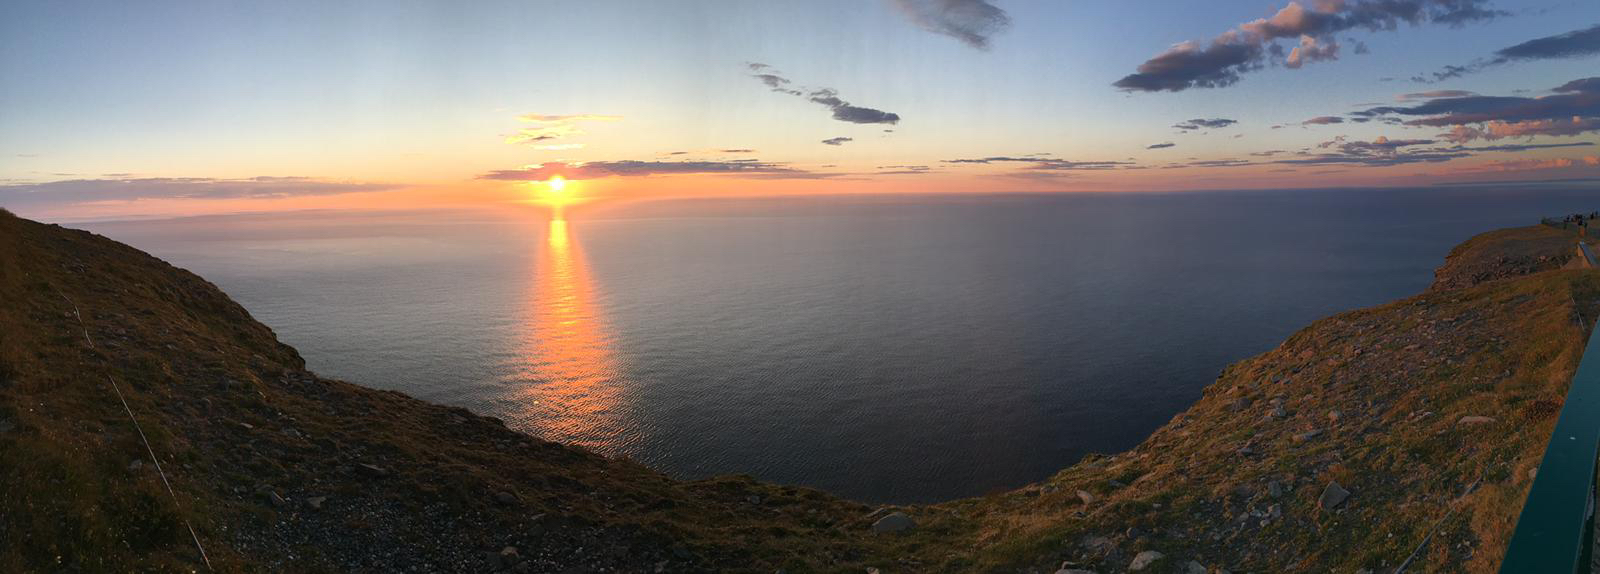
\includegraphics[width=2\textwidth]{images/sonne-meer}}%
  [A doublepage image with a caption on the right side of the right part.]%
  {A caption for a double-sided image that will be placed on the right side of the
   right-hand part of the illustration. The illustration begins on the left edge of 
   the paper. A short form is used for the LOF. 
   The parameter is \texttt{doublePage}}%
  {fig:doublePage0a}
\end{lstlisting}


\marginnote{Fig. \ref{fig:doublePage0a}}
\hvFloat[doublePage,capWidth=n,capPos=right]%
  {figure}%
  {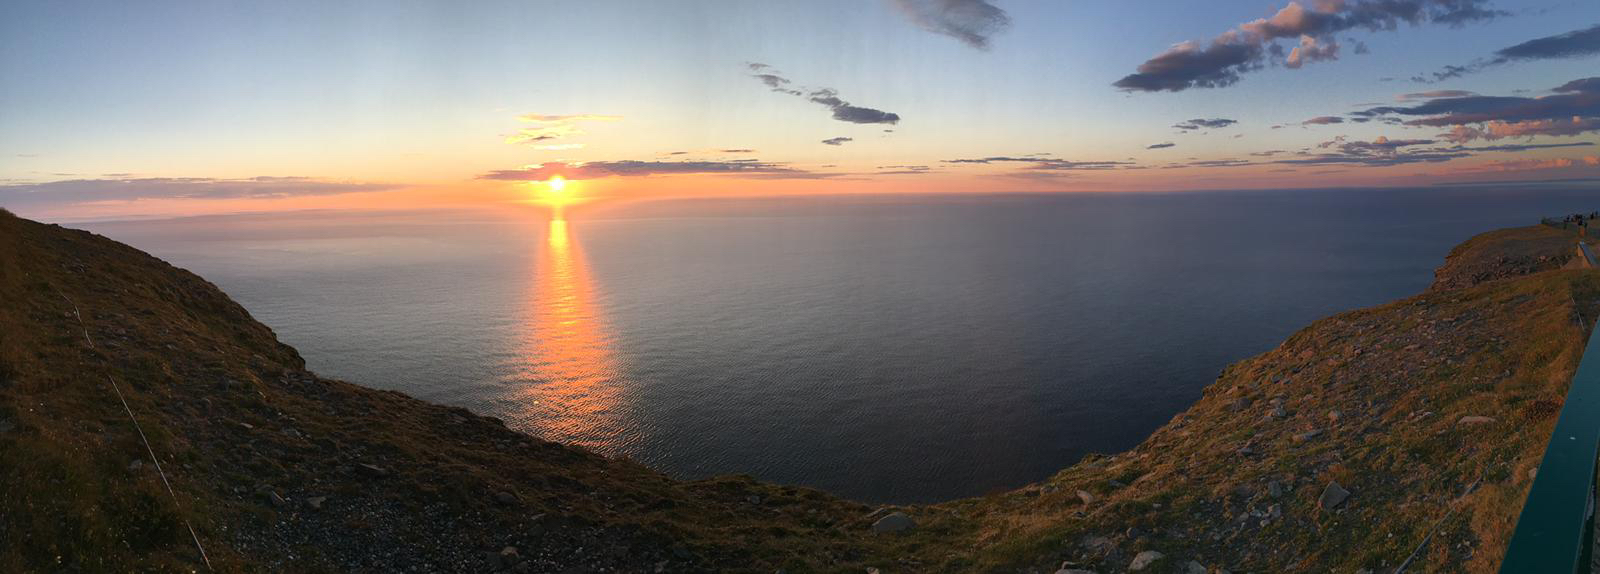
\includegraphics[width=2\textwidth]{images/sonne-meer}}%
  [A doublepage image with a caption on the right side of the right part.]%
  {A caption for a double-sided image that will be placed on the right side of the
   right-hand part of the illustration. The illustration begins on the left edge of 
   the paper. A short form is used for the LOF. 
   The parameter is \texttt{doublePage}}%
  {fig:doublePage0a}


\hvblindtext

\Blindtext

\Blindtext

\Blindtext




\subsubsection{\texttt{bindCorr=1cm}}

\begin{lstlisting}
\hvFloat[doublePage,capWidth=n,capPos=right,bindCorr=1cm]%
  {figure}%
  {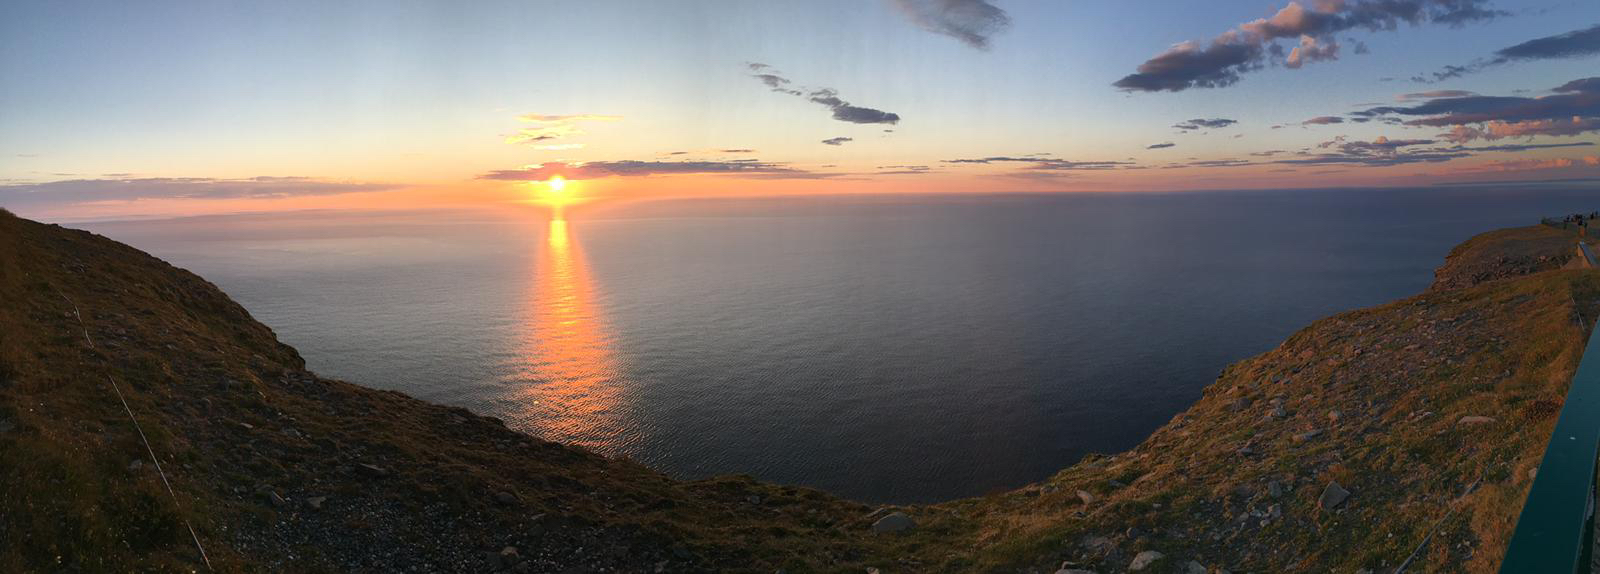
\includegraphics[width=2\textwidth]{images/sonne-meer}}%
  [A doublepage image with a caption on the right side of the right part.]%
  {A caption for a double-sided image that will be placed on the right side of the
   right-hand part of the illustration. The illustration begins on the left edge of 
   the paper. A short form is used for the LOF. 
   The parameter is \texttt{doublePage}}%
  {fig:doublePage1a}
\end{lstlisting}

\marginnote{Fig. \ref{fig:doublePage1a}}
\hvFloat[doublePage,capWidth=n,capPos=right,bindCorr=1cm]%
  {figure}%
  {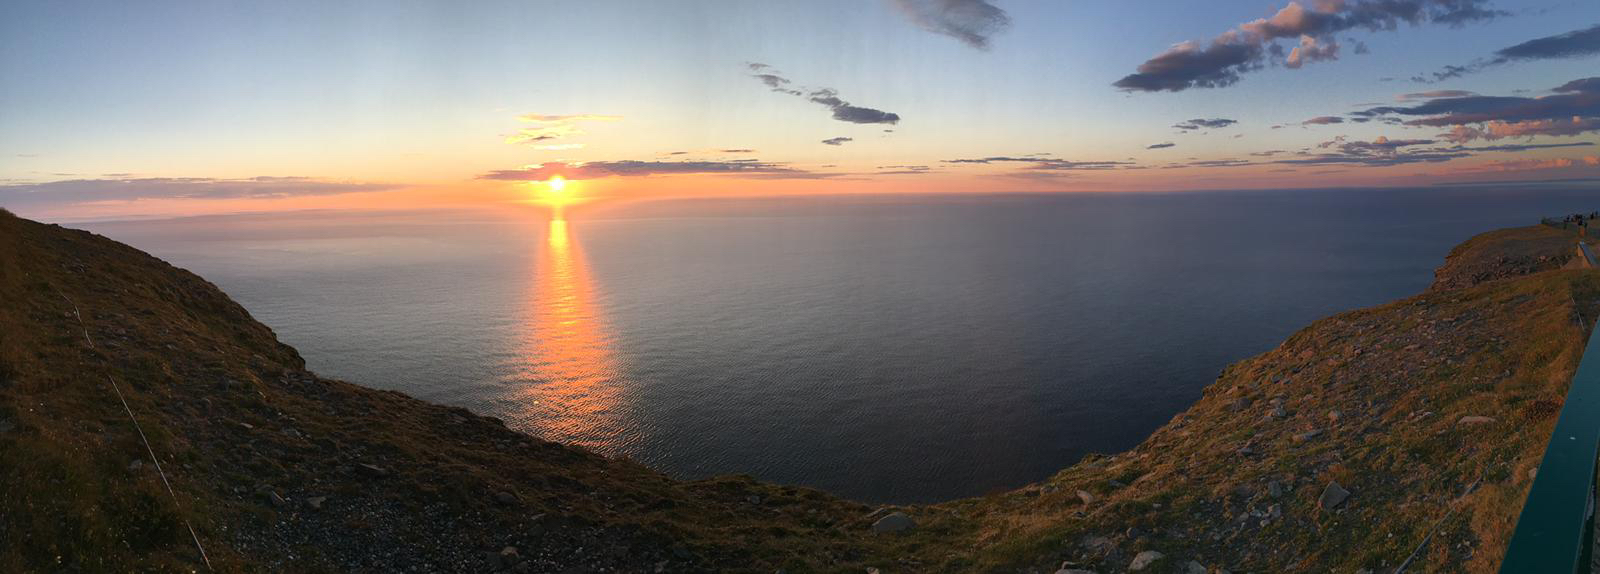
\includegraphics[width=2\textwidth]{images/sonne-meer}}%
  [A doublepage image with a caption on the right side of the right part.]%
  {A caption for a double-sided image that will be placed on the right side of the
   right-hand part of the illustration. The illustration begins on the left edge of 
   the paper. A short form is used for the LOF. 
   The parameter is \texttt{doublePage}}%
  {fig:doublePage1a}

\hvblindtext

\Blindtext

\Blindtext

\Blindtext

\hvblindtext

\subsubsection{\texttt{bindCorr=3mm}}

\begin{lstlisting}
\hvFloat[doublePage,capWidth=n,capPos=right,bindCorr=3mm]%
  {figure}%
  {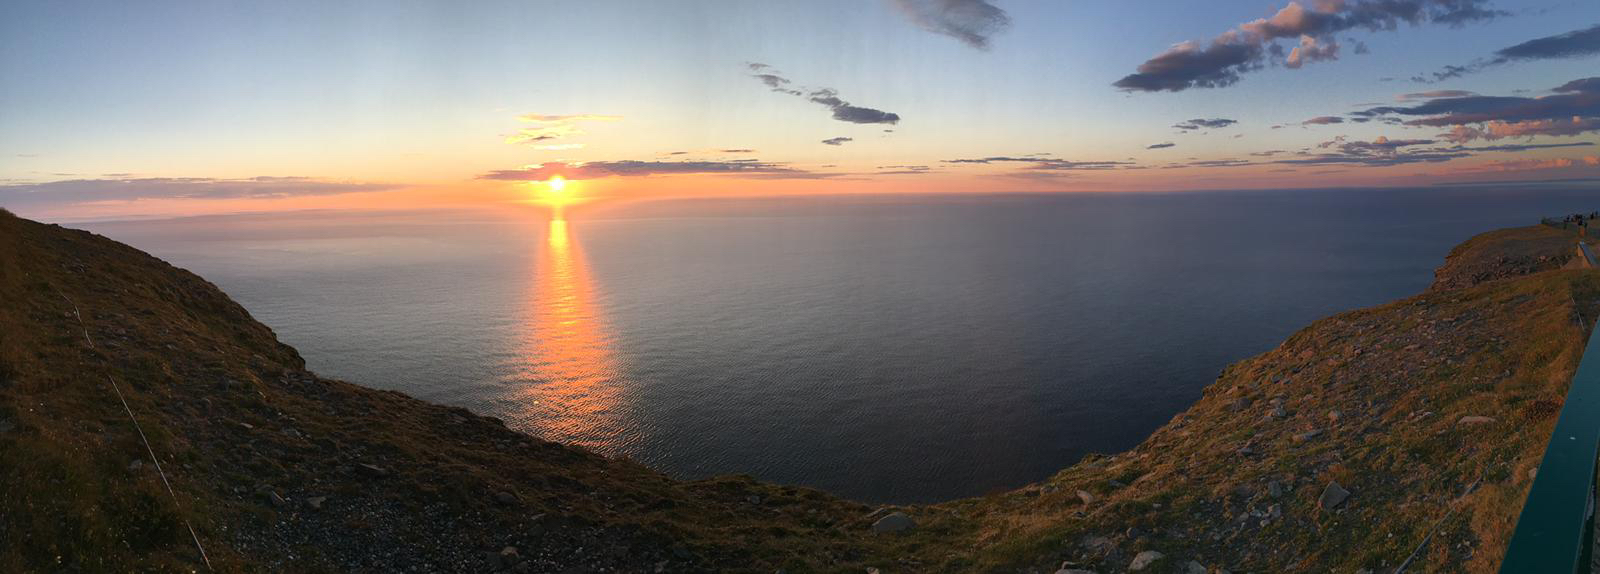
\includegraphics[width=2\textwidth]{images/sonne-meer}}%
  [A doublepage image with a caption on the right side of the right part.]%
  {A caption for a double-sided image that will be placed on the right side of the
   right-hand part of the illustration. The illustration begins on the left edge of 
   the paper. A short form is used for the LOF. 
   The parameter is \texttt{doublePage}}%
  {fig:doublePage2a}
\end{lstlisting}

\marginnote{Fig. \ref{fig:doublePage2a}}
\hvFloat[doublePage,capWidth=n,capPos=right,bindCorr=3mm]%
  {figure}%
  {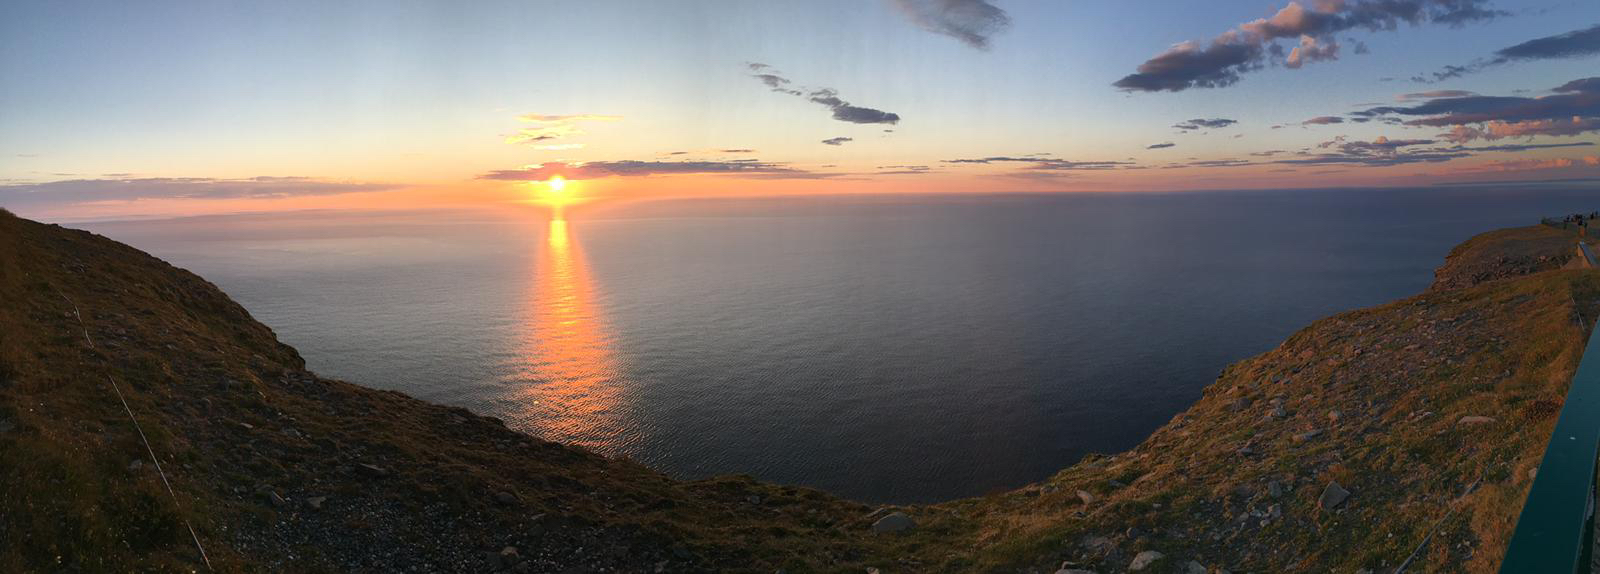
\includegraphics[width=2\textwidth]{images/sonne-meer}}%
  [A doublepage image with a caption on the right side of the right part.]%
  {A caption for a double-sided image that will be placed on the right side of the
   right-hand part of the illustration. The illustration begins on the left edge of 
   the paper. A short form is used for the LOF. 
   The parameter is \texttt{doublePage}}%
  {fig:doublePage2a}


\Blindtext

\Blindtext

\Blindtext

\hvblindtext

\subsubsection{\texttt{bindCorr=<inside textwidth>}}

\begin{lstlisting}
\hvFloat[doublePage,capWidth=n,bindCorr=\the\dimexpr1in+\oddsidemargin]%
  {figure}%
  {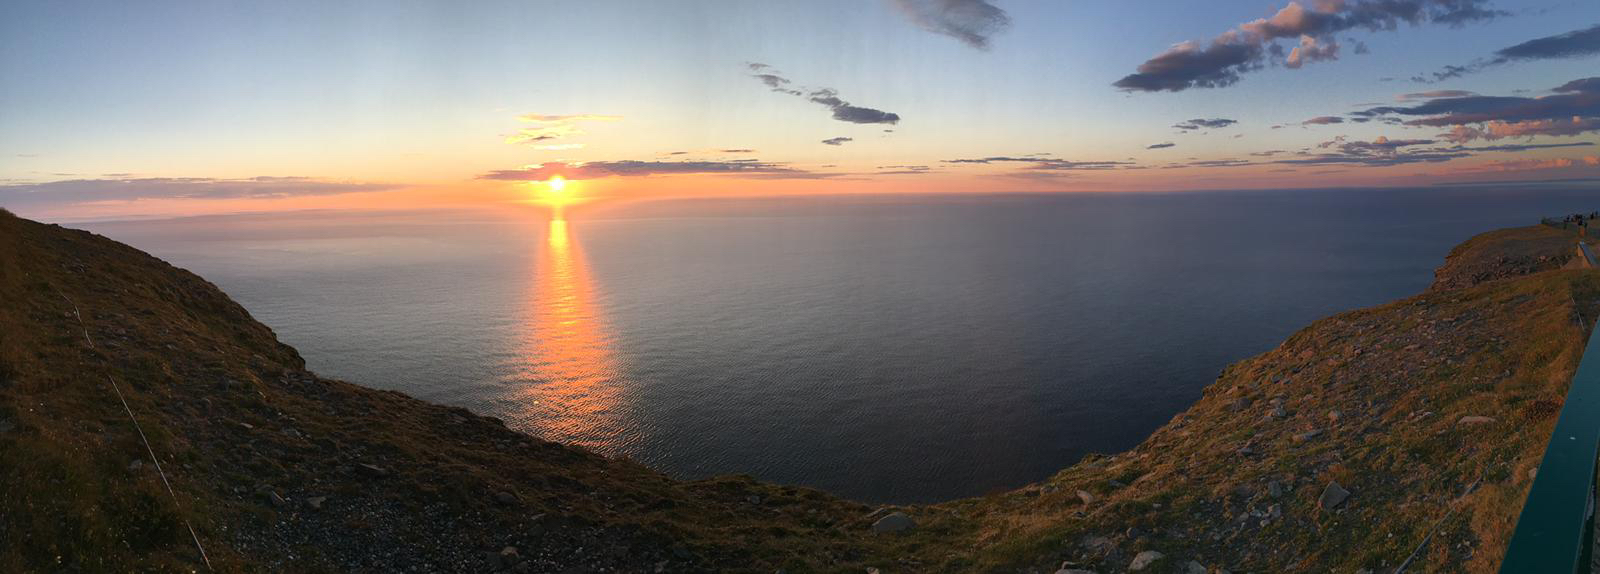
\includegraphics[width=2\textwidth]{images/sonne-meer}}%
  [A doublepage image with a caption on the right side of the right part.]%
  {A caption for a double-sided image that will be placed on the right side of the
   right-hand part of the illustration. The illustration begins on the left edge of 
   the paper. A short form is used for the LOF. 
   The parameter is \texttt{doublePage}}%
  {fig:doublePage3a}
\end{lstlisting}

\marginnote{Fig. \ref{fig:doublePage3a}}
\hvFloat[doublePage,capWidth=n,bindCorr=\the\dimexpr1in+\oddsidemargin]%
  {figure}%
  {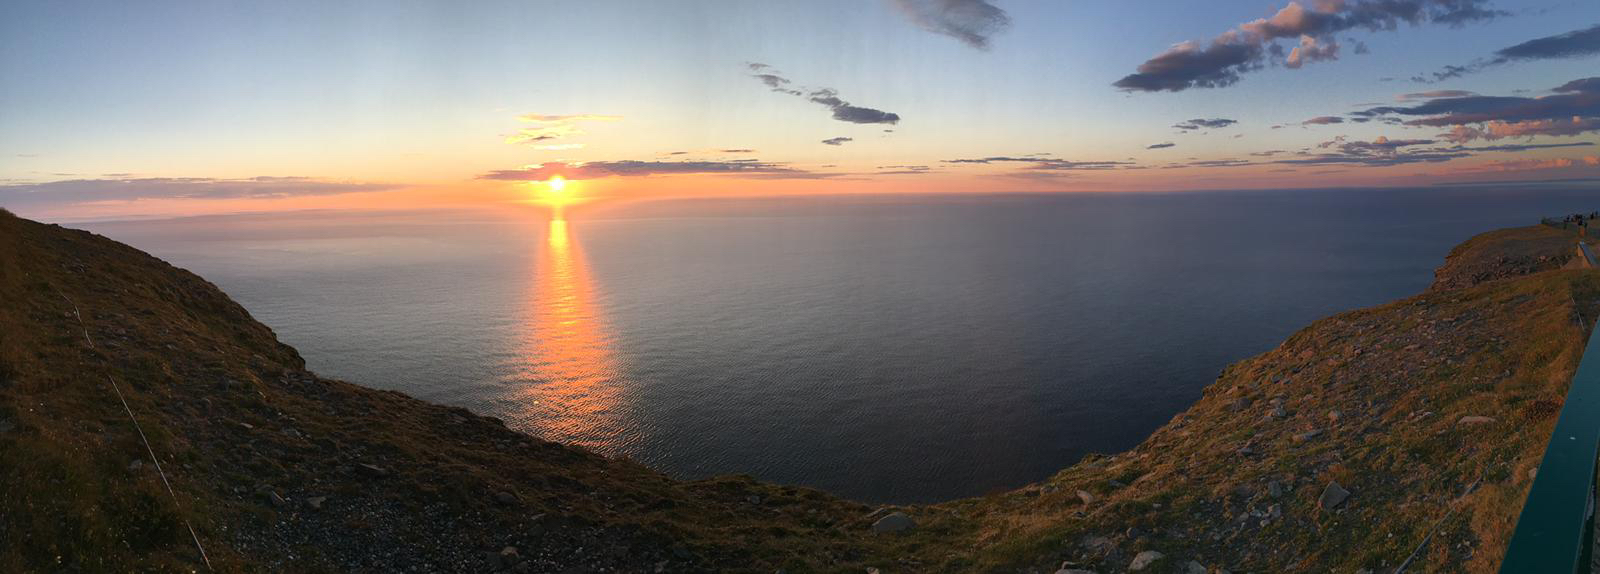
\includegraphics[width=2\textwidth]{images/sonne-meer}}%
  [A doublepage image with a caption on the right side of the right part.]%
  {A caption for a double-sided image that will be placed on the right side of the
   right-hand part of the illustration. The illustration begins on the left edge of 
   the paper. A short form is used for the LOF. 
   The parameter is \texttt{doublePage}}%
  {fig:doublePage3a}


\Blindtext

\Blindtext

\Blindtext



\clearpage

\section{Argument \texttt{doublePAGE}}
\subsection{Definition on an odd page}

\Blindtext

\hvblindtext

\subsubsection{The default}

\begin{lstlisting}
\hvFloat[doublePAGE,capWidth=n,capPos=right]%
  {figure}%
  {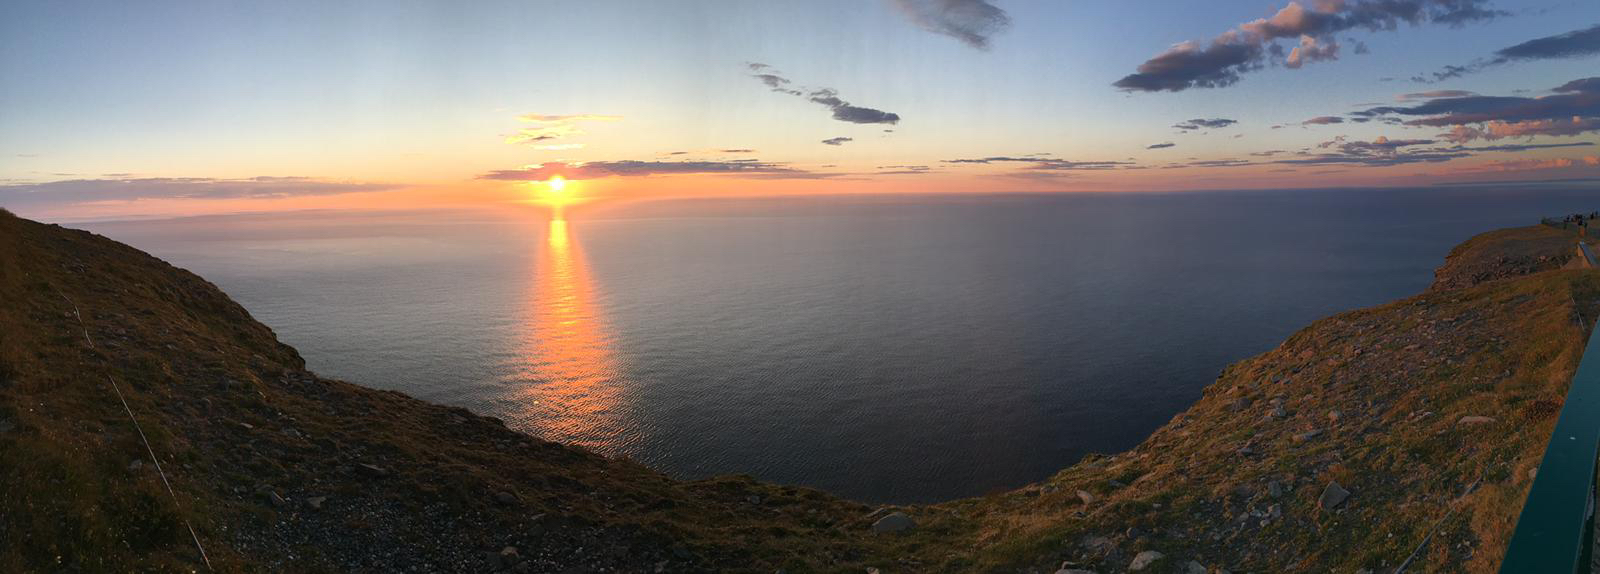
\includegraphics[width=2\textwidth]{images/sonne-meer}}%
  [A doublepage image with a caption on the right side of the right part.]%
  {A caption for a double-sided image that will be placed on the right side of the
   right-hand part of the illustration. The illustration begins on the left edge of 
   the paper. A short form is used for the LOF. 
   The parameter is \texttt{doublePAGE}}%
  {fig:doublePAGE0}
\end{lstlisting}


\marginnote{Fig. \ref{fig:doublePAGE0}}
\hvFloat[doublePAGE,capWidth=n,capPos=right]%
  {figure}%
  {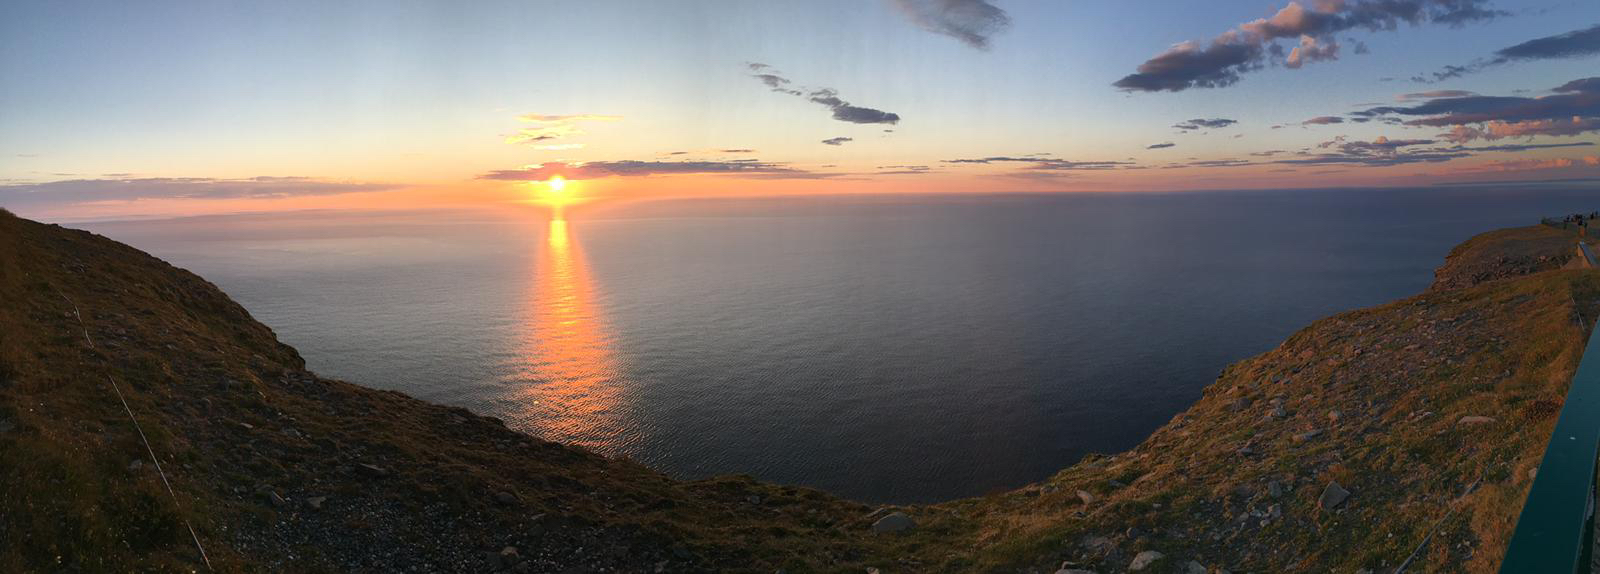
\includegraphics[width=2\textwidth]{images/sonne-meer}}%
  [A doublepage image with a caption on the right side of the right part.]%
  {A caption for a double-sided image that will be placed on the right side of the
   right-hand part of the illustration. The illustration begins on the left edge of 
   the paper. A short form is used for the LOF. 
   The parameter is \texttt{doublePAGE}}%
  {fig:doublePAGE0}

\Blindtext

\Blindtext

\hvblindtext

\subsubsection{\texttt{bindCorr=1cm}}

\begin{lstlisting}
\hvFloat[doublePAGE,capWidth=n,capPos=right,bindCorr=1cm]%
  {figure}%
  {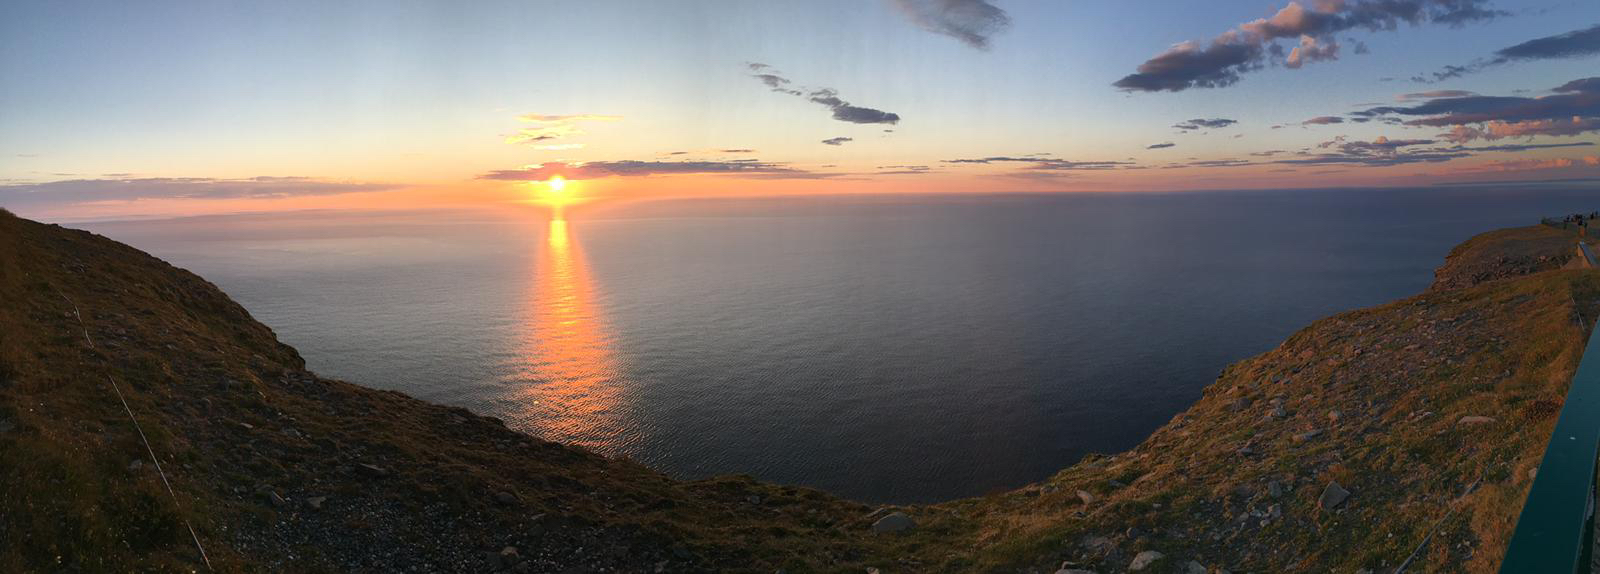
\includegraphics[width=2\textwidth]{images/sonne-meer}}%
  [A doublepage image with a caption on the right side of the right part.]%
  {A caption for a double-sided image that will be placed on the right side of the
   right-hand part of the illustration. The illustration begins on the left edge of 
   the paper. A short form is used for the LOF. 
   The parameter is \texttt{doublePAGE}}%
  {fig:doublePAGE1}
\end{lstlisting}

\marginnote{Fig. \ref{fig:doublePAGE1}}
\hvFloat[doublePAGE,capWidth=n,capPos=right,bindCorr=1cm]%
  {figure}%
  {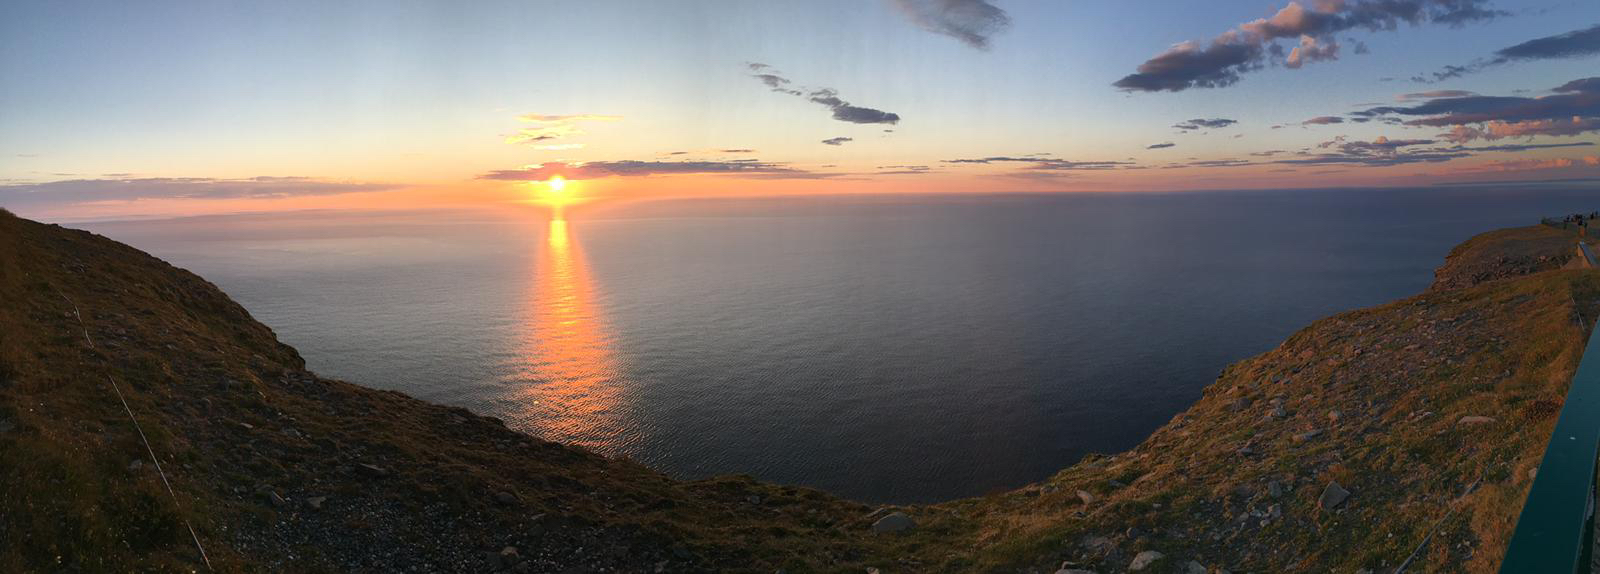
\includegraphics[width=2\textwidth]{images/sonne-meer}}%
  [A doublepage image with a caption on the right side of the right part.]%
  {A caption for a double-sided image that will be placed on the right side of the
   right-hand part of the illustration. The illustration begins on the left edge of 
   the paper. A short form is used for the LOF. 
   The parameter is \texttt{doublePAGE}}%
  {fig:doublePAGE1}

\hvblindtext

\Blindtext

\Blindtext

\subsubsection{\texttt{bindCorr=3mm}}

\begin{lstlisting}
\hvFloat[doublePAGE,capWidth=n,capPos=right,bindCorr=3mm]%
  {figure}%
  {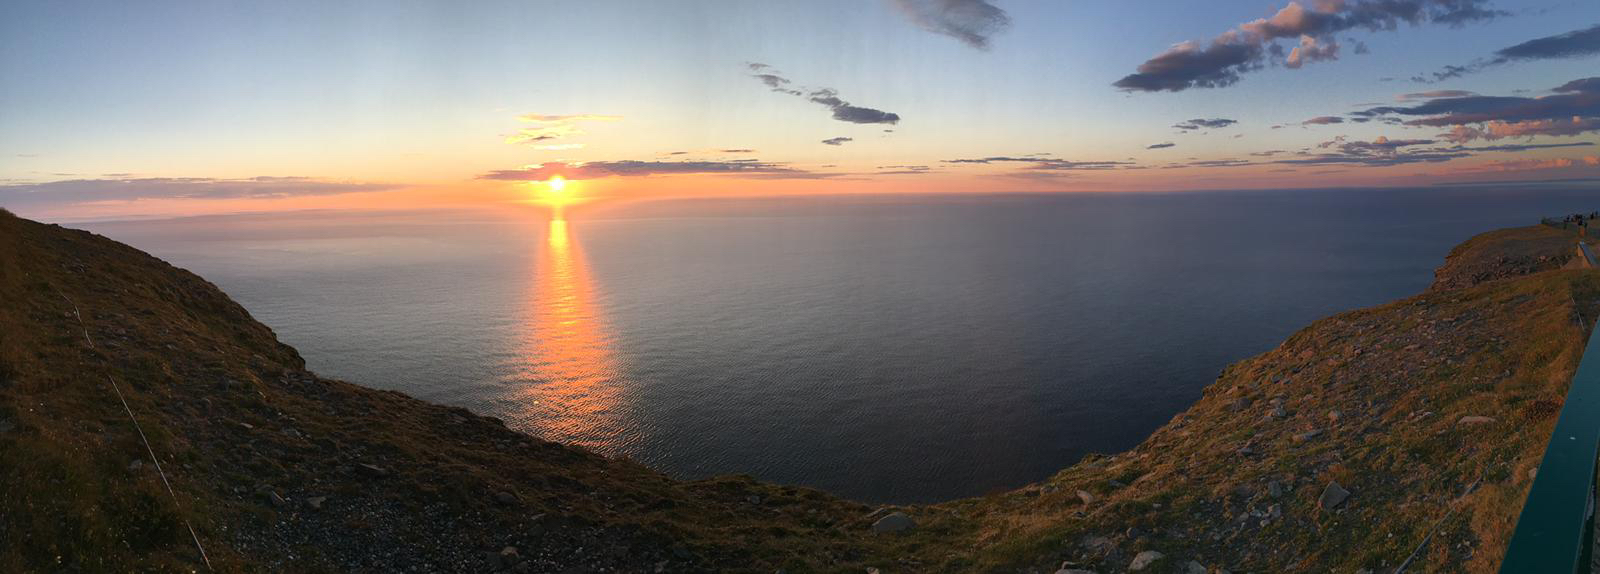
\includegraphics[width=2\textwidth]{images/sonne-meer}}%
  [A doublepage image with a caption on the right side of the right part.]%
  {A caption for a double-sided image that will be placed on the right side of the
   right-hand part of the illustration. The illustration begins on the left edge of 
   the paper. A short form is used for the LOF. 
   The parameter is \texttt{doublePAGE}}%
  {fig:doublePAGE2}
\end{lstlisting}

\marginnote{Fig. \ref{fig:doublePAGE2}}
\hvFloat[doublePAGE,capWidth=n,capPos=right,bindCorr=3mm]%
  {figure}%
  {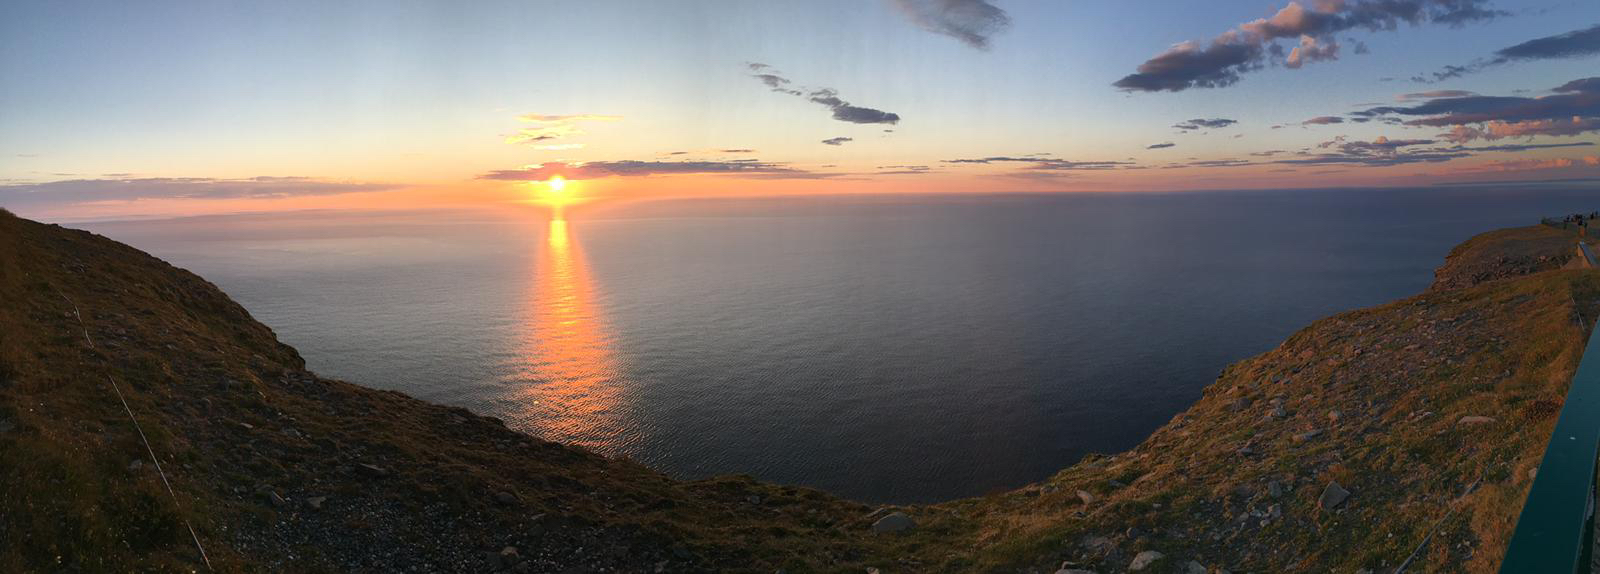
\includegraphics[width=2\textwidth]{images/sonne-meer}}%
  [A doublepage image with a caption on the right side of the right part.]%
  {A caption for a double-sided image that will be placed on the right side of the
   right-hand part of the illustration. The illustration begins on the left edge of 
   the paper. A short form is used for the LOF. 
   The parameter is \texttt{doublePAGE}}%
  {fig:doublePAGE2}



\Blindtext

\Blindtext

\hvblindtext

\hvblindtext

\subsubsection{\texttt{bindCorr=<inside textwidth>}}

\begin{lstlisting}
\hvFloat[doublePAGE,capWidth=n,bindCorr=\the\dimexpr1in+\oddsidemargin]%
  {figure}%
  {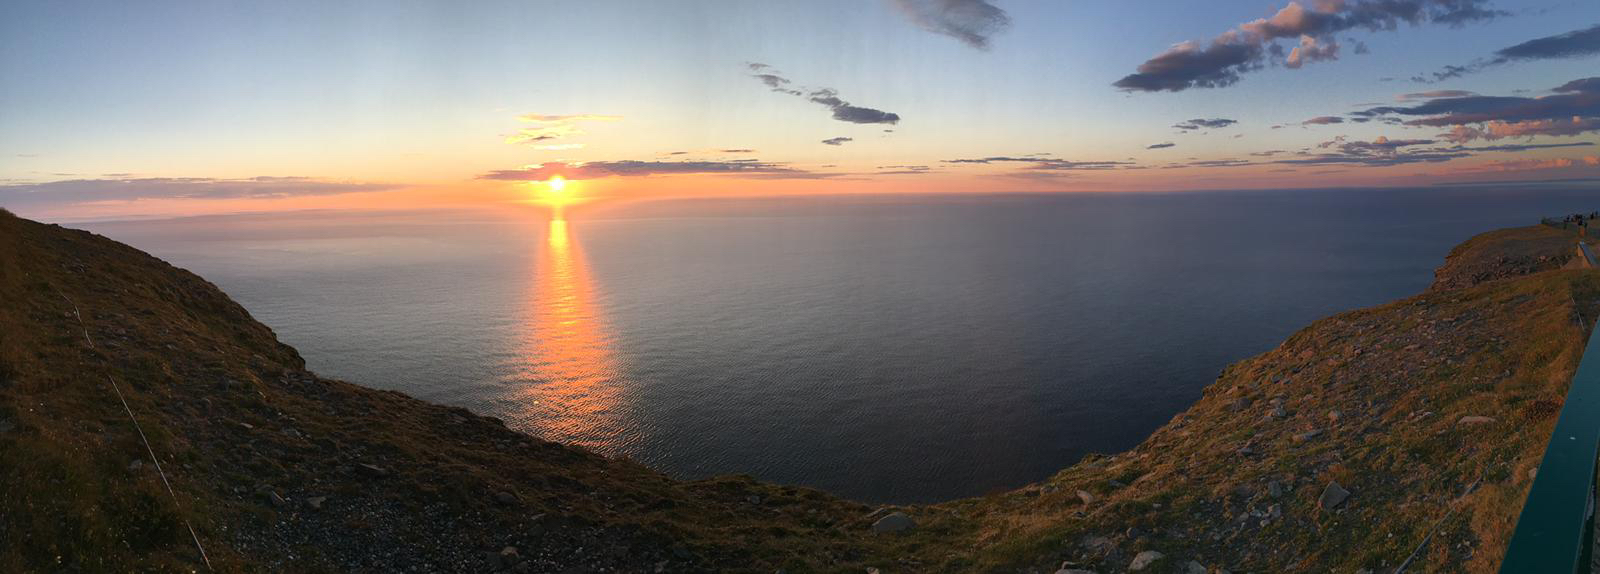
\includegraphics[width=2\textwidth]{images/sonne-meer}}%
  [A doublepage image with a caption on the right side of the right part.]%
  {A caption for a double-sided image that will be placed on the right side of the
   right-hand part of the illustration. The illustration begins on the left edge of 
   the paper. A short form is used for the LOF. 
   The parameter is \texttt{doublePAGE}}%
  {fig:doublePAGE3}
\end{lstlisting}

\marginnote{Fig. \ref{fig:doublePAGE3}}
\hvFloat[doublePAGE,capWidth=n,bindCorr=\the\dimexpr1in+\oddsidemargin]%
  {figure}%
  {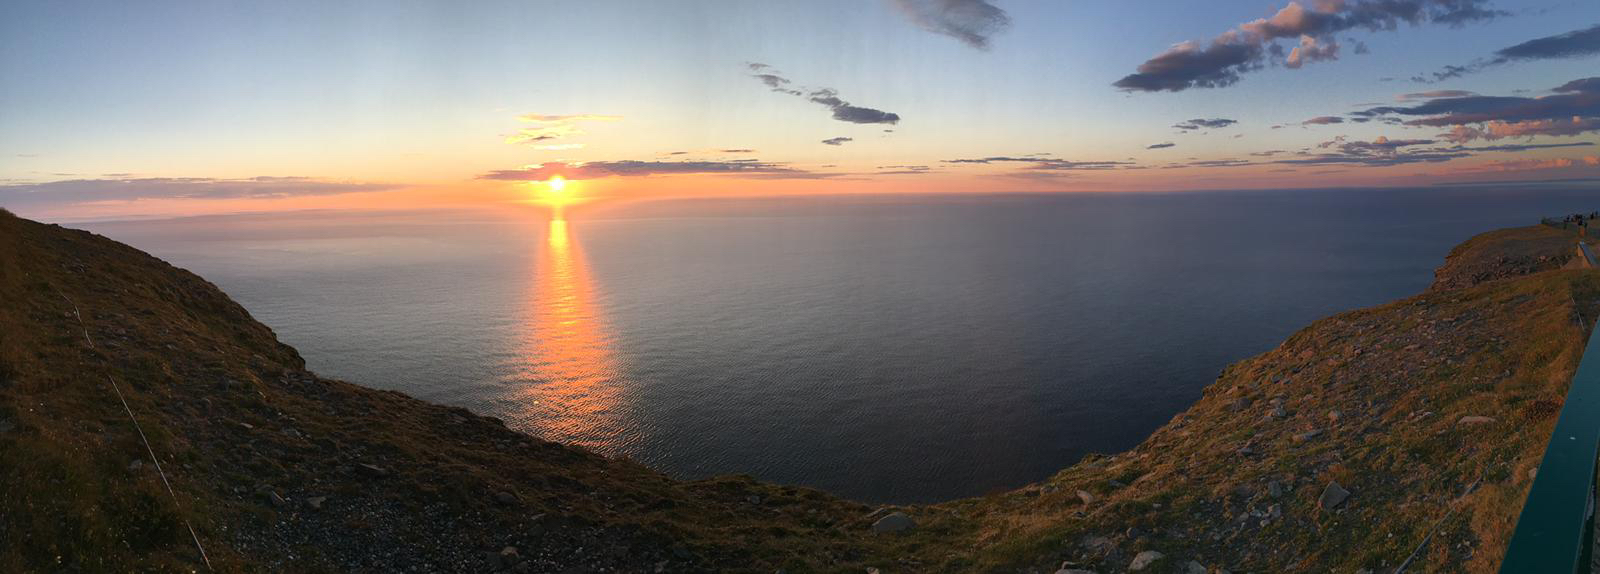
\includegraphics[width=2\textwidth]{images/sonne-meer}}%
  [A doublepage image with a caption on the right side of the right part.]%
  {A caption for a double-sided image that will be placed on the right side of the
   right-hand part of the illustration. The illustration begins on the left edge of 
   the paper. A short form is used for the LOF. 
   The parameter is \texttt{doublePAGE}}%
  {fig:doublePAGE3}


%\hvblindtext

\Blindtext


\subsection{Definition on an even page}


\subsubsection{The default}

\begin{lstlisting}
\hvFloat[doublePAGE,capWidth=n,capPos=right]{figure}%
  {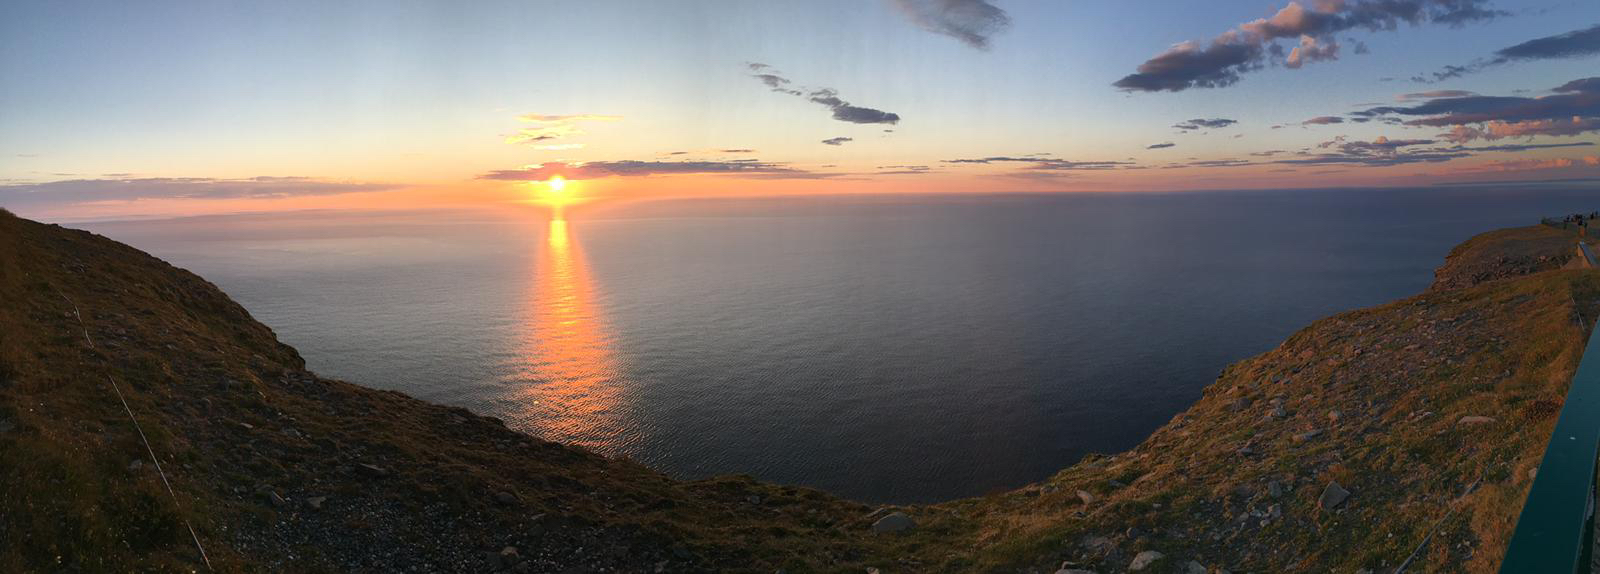
\includegraphics[width=2\textwidth]{images/sonne-meer}}%
  [A doublepage image with a caption on the right side of the right part.]%
  {A caption for a double-sided image that will be placed on the right side of the
   right-hand part of the illustration. The illustration begins on the left edge of 
   the paper. A short form is used for the LOF. 
   The parameter is \texttt{doublePAGE}}%
  {fig:doublePAGE0a}
\end{lstlisting}


\marginnote{Fig. \ref{fig:doublePAGE0a}}
\hvFloat[doublePAGE,capWidth=n,capPos=right]%
  {figure}%
  {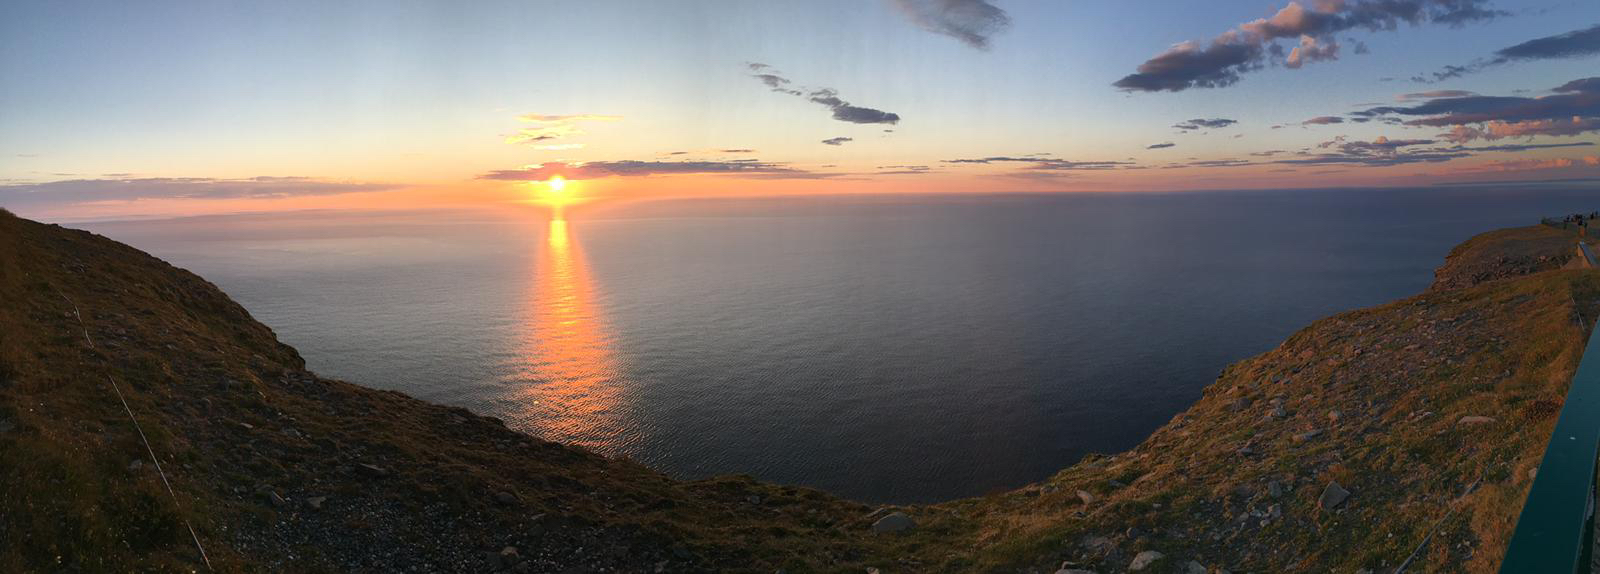
\includegraphics[width=2\textwidth]{images/sonne-meer}}%
  [A doublepage image with a caption on the right side of the right part.]%
  {A caption for a double-sided image that will be placed on the right side of the
   right-hand part of the illustration. The illustration begins on the left edge of 
   the paper. A short form is used for the LOF. 
   The parameter is \texttt{doublePAGE}}%
  {fig:doublePAGE0a}

\Blindtext

\Blindtext

\hvblindtext

\subsubsection{\texttt{bindCorr=1cm}}

\begin{lstlisting}
\hvFloat[doublePAGE,capWidth=n,capPos=right,bindCorr=1cm]%
  {figure}%
  {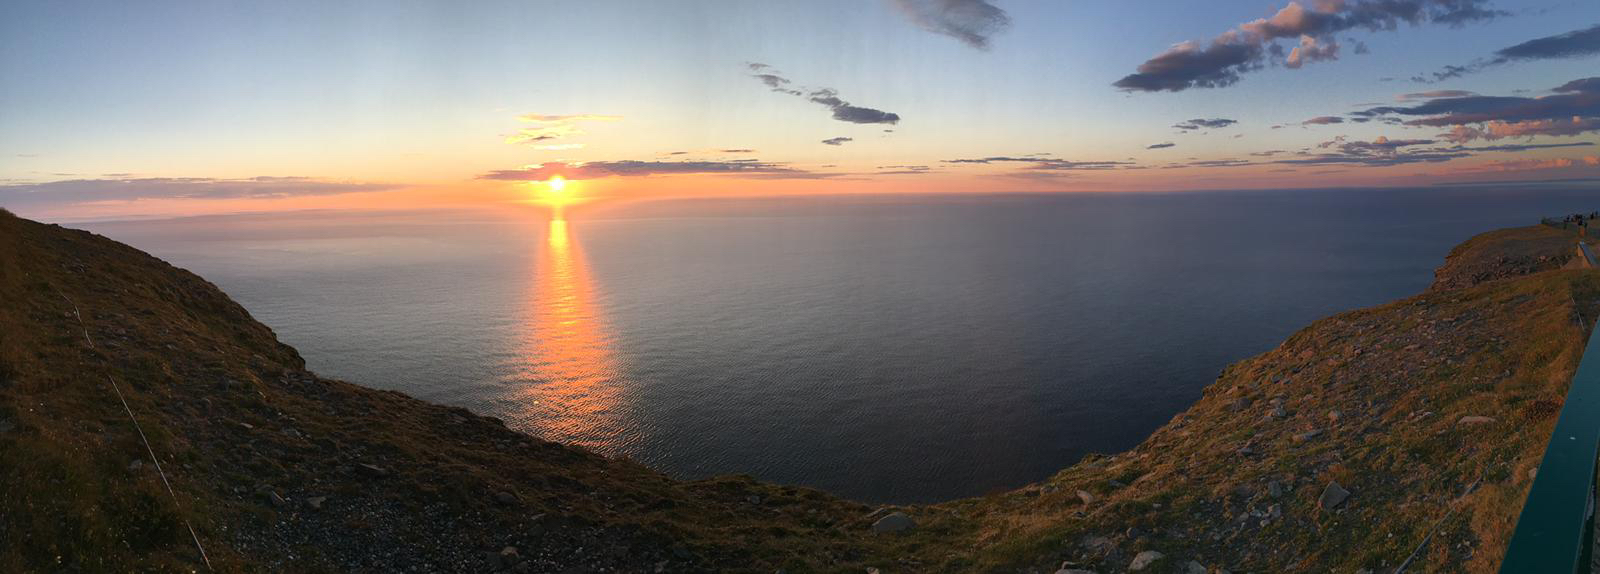
\includegraphics[width=2\textwidth]{images/sonne-meer}}%
  [A doublepage image with a caption on the right side of the right part.]%
  {A caption for a double-sided image that will be placed on the right side of the
   right-hand part of the illustration. The illustration begins on the left edge of 
   the paper. A short form is used for the LOF. 
   The parameter is \texttt{doublePAGE}}%
  {fig:doublePAGE1a}
\end{lstlisting}

\marginnote{Fig. \ref{fig:doublePAGE1a}}
\hvFloat[doublePAGE,capWidth=n,capPos=right,bindCorr=1cm]%
  {figure}%
  {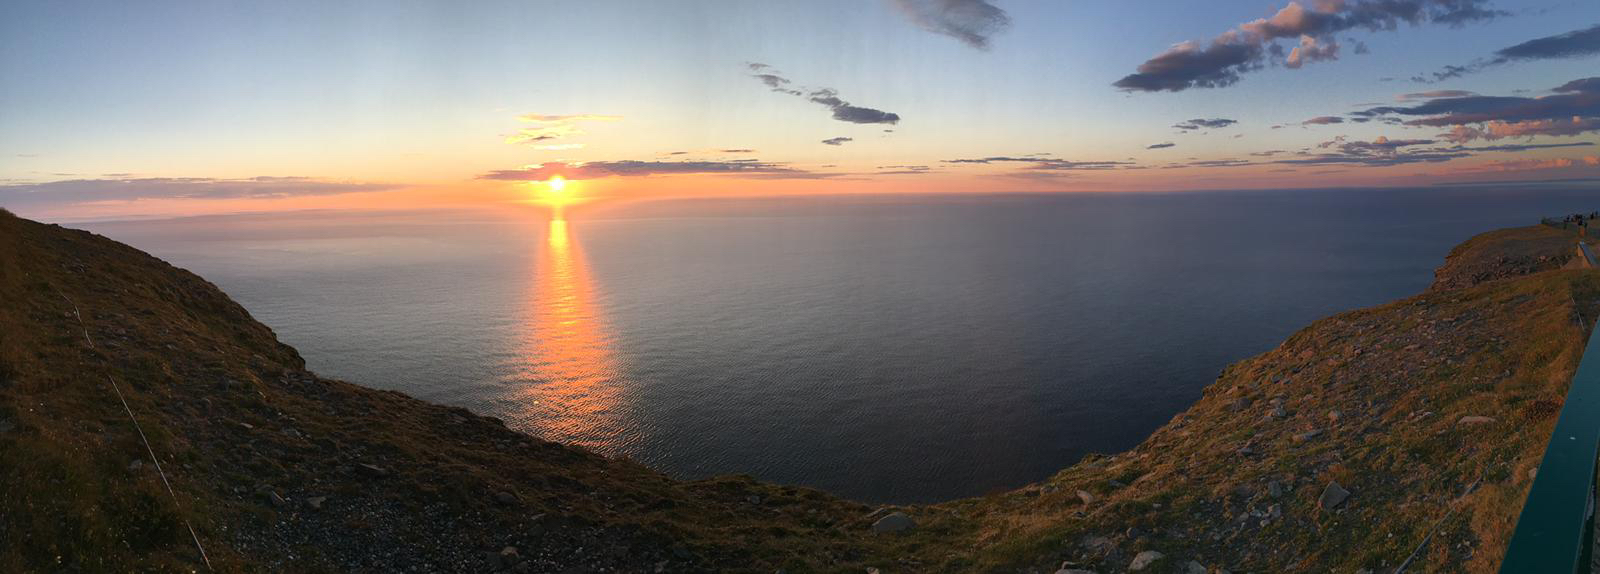
\includegraphics[width=2\textwidth]{images/sonne-meer}}%
  [A doublepage image with a caption on the right side of the right part.]%
  {A caption for a double-sided image that will be placed on the right side of the
   right-hand part of the illustration. The illustration begins on the left edge of 
   the paper. A short form is used for the LOF. 
   The parameter is \texttt{doublePAGE}}%
  {fig:doublePAGE1a}

\hvblindtext

\Blindtext

\Blindtext

\subsubsection{\texttt{bindCorr=3mm}}

\begin{lstlisting}
\hvFloat[doublePAGE,capWidth=n,capPos=right,bindCorr=3mm]%
  {figure}%
  {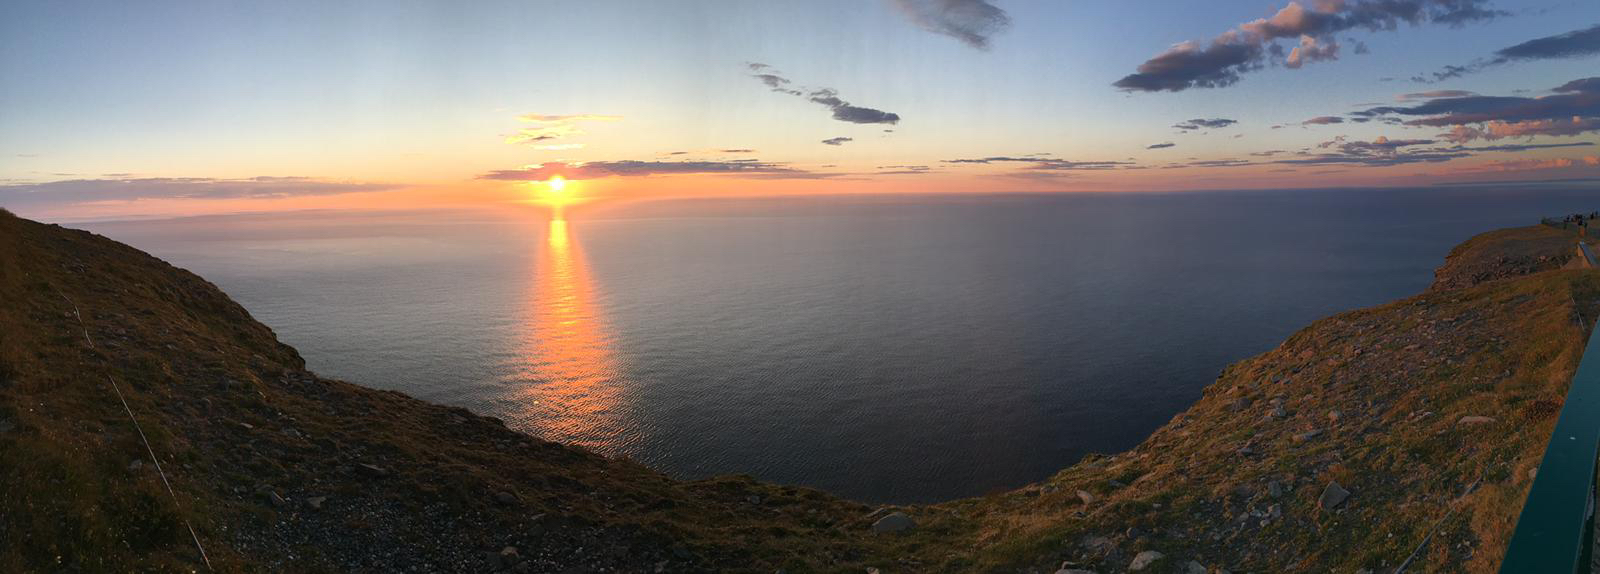
\includegraphics[width=2\textwidth]{images/sonne-meer}}%
  [A doublepage image with a caption on the right side of the right part.]%
  {A caption for a double-sided image that will be placed on the right side of the
   right-hand part of the illustration. The illustration begins on the left edge of 
   the paper. A short form is used for the LOF. 
   The parameter is \texttt{doublePAGE}}%
  {fig:doublePAGE2a}
\end{lstlisting}

\marginnote{Fig. \ref{fig:doublePAGE2a}}
\hvFloat[doublePAGE,capWidth=n,capPos=right,bindCorr=3mm]%
  {figure}%
  {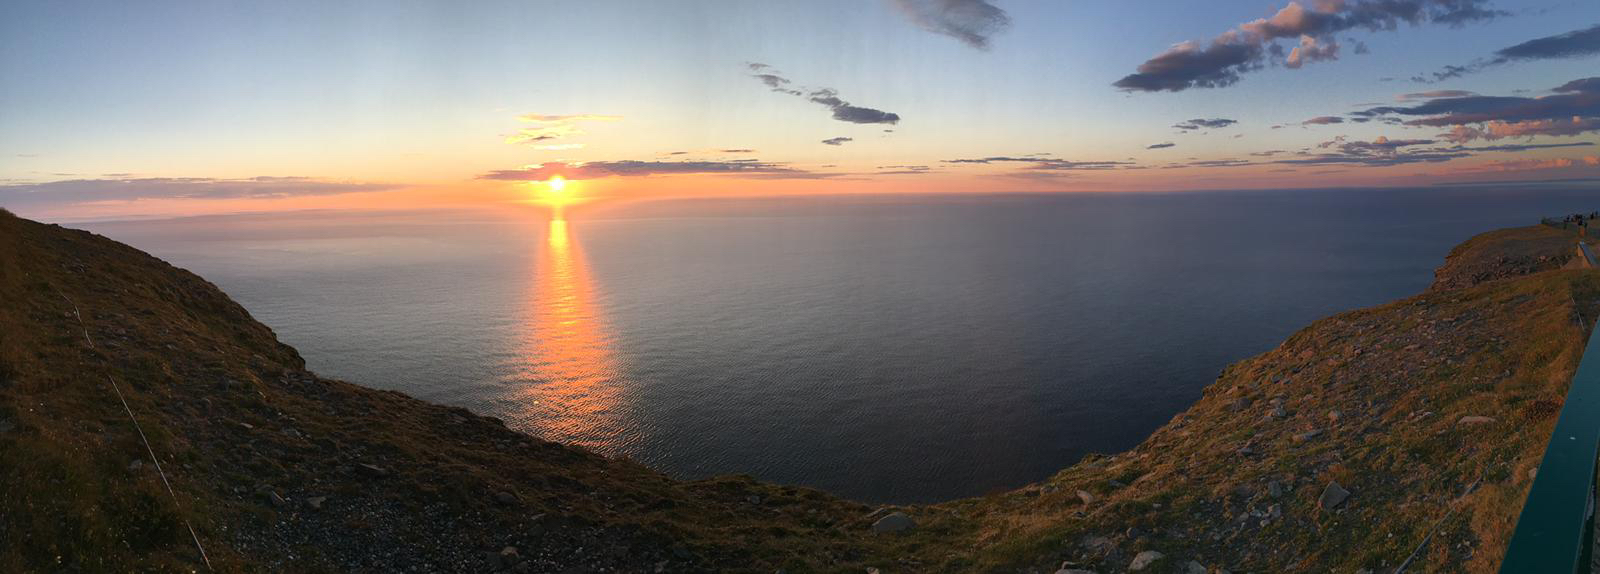
\includegraphics[width=2\textwidth]{images/sonne-meer}}%
  [A doublepage image with a caption on the right side of the right part.]%
  {A caption for a double-sided image that will be placed on the right side of the
   right-hand part of the illustration. The illustration begins on the left edge of 
   the paper. A short form is used for the LOF. 
   The parameter is \texttt{doublePAGE}}%
  {fig:doublePAGE2a}



\Blindtext

\Blindtext

\hvblindtext
\subsubsection{\texttt{bindCorr=<inside textwidth>}}

\begin{lstlisting}
\hvFloat[doublePAGE,capWidth=n,bindCorr=\the\dimexpr1in+\oddsidemargin]%
  {figure}%
  {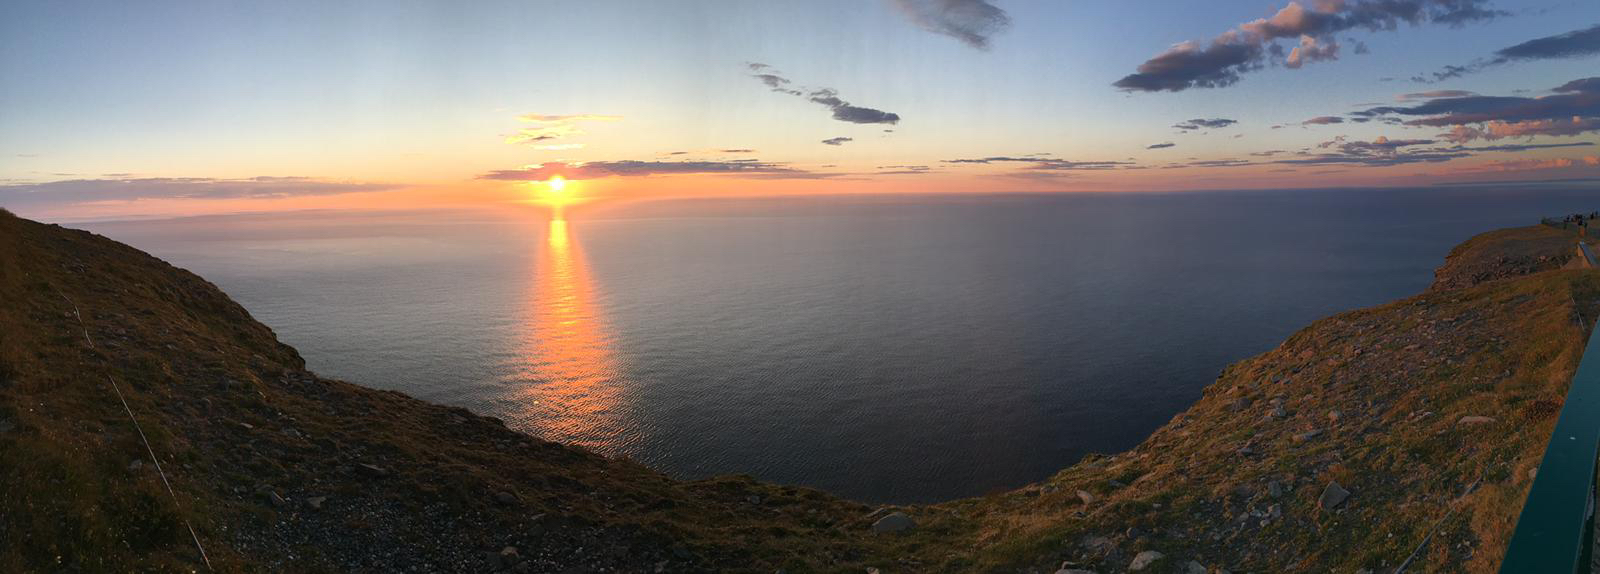
\includegraphics[width=2\textwidth]{images/sonne-meer}}%
  [A doublepage image with a caption on the right side of the right part.]%
  {A caption for a double-sided image that will be placed on the right side of the
   right-hand part of the illustration. The illustration begins on the left edge of 
   the paper. A short form is used for the LOF. 
   The parameter is \texttt{doublePAGE}}%
  {fig:doublePAGE3a}
\end{lstlisting}

\marginnote{Fig. \ref{fig:doublePAGE3a}}
\hvFloat[doublePAGE,capWidth=n,bindCorr=\the\dimexpr1in+\oddsidemargin]%
  {figure}%
  {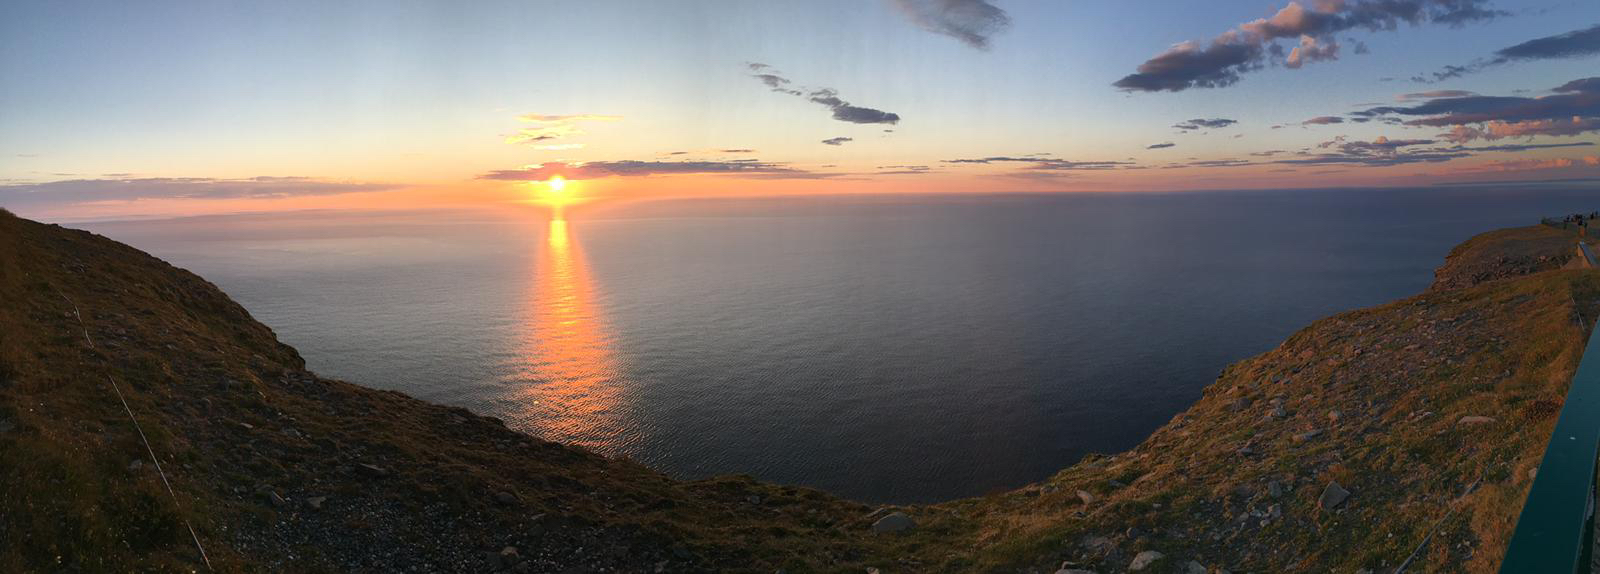
\includegraphics[width=2\textwidth]{images/sonne-meer}}%
  [A doublepage image with a caption on the right side of the right part.]%
  {A caption for a double-sided image that will be placed on the right side of the
   right-hand part of the illustration. The illustration begins on the left edge of 
   the paper. A short form is used for the LOF. 
   The parameter is \texttt{doublePAGE}}%
  {fig:doublePAGE3a}


\Blindtext

\Blindtext


\section{Argument \texttt{doubleFULLPAGE}}
\subsection{Definition on an odd page}

\Blindtext
\hvblindtext

\subsubsection{The default}

\begin{lstlisting}
\hvFloat[doubleFULLPAGE,capWidth=n,capFormat={labelfont=sf,font=sf,format=plain}]%
  {figure}%
  {\includegraphics[doubleFULLPAGE]{images/rheinsberg}}%
  [A doublepage image with a caption on the right side of the right part.]%
  {A caption for a double-sided image that will be placed on the right side of the
   right-hand part of the illustration. The illustration begins on the left edge of 
   the paper. A short form is used for the LOF. 
   The parameter is \texttt{doubleFULLPAGE}}%
  {fig:doubleFULLPAGE0}
\end{lstlisting}


\marginnote{Fig. \ref{fig:doubleFULLPAGE0}}
\hvFloat[doubleFULLPAGE,capWidth=n,capFormat={labelfont=sf,font=sf,format=plain}]%
  {figure}%
  {\includegraphics[doubleFULLPAGE]{images/rheinsberg}}%
  [A doublepage image with a caption on the right side of the right part.]%
  {A caption for a double-sided image that will be placed on the right side of the
   right-hand part of the illustration. The illustration begins on the left edge of 
   the paper. A short form is used for the LOF. 
   The parameter is \texttt{doubleFULLPAGE}}%
  {fig:doubleFULLPAGE0}

\Blindtext

\Blindtext

\hvblindtext


\subsubsection{Caption \emph{before} doublepage image}
The caption of image~\ref{fig:doubleFULLPAGE0before-cap} (internal label \texttt{fig:doubleFULLPAGE0before-cap}) is on 
page~\pageref{fig:doubleFULLPAGE0before-cap} and the first page of the image 
is on the page~\pageref{fig:doubleFULLPAGE0before} (main label \texttt{fig:doubleFULLPAGE0before}) and the
second (right) part  is on page~\pageref{fig:doubleFULLPAGE0before-2} (internal label \texttt{fig:doubleFULLPAGE0before-2}).

\begin{lstlisting}
\hvFloat[doubleFULLPAGE,capWidth=n,capFormat={labelfont=sf,font=sf,format=plain},capPos=before,separatorLine]%
  {figure}%
  {\includegraphics[doubleFULLPAGE]{images/rheinsberg}}%
  [A doublepage image with a caption before the double page image on the bottom of the page.]%
  {A caption for a double-sided image that will be placed on the bottom of the page and before
   the doublepage illustration. The illustration begins o4n the left edge of 
   the paper. A short form is used for the LOF. 
   The parameter is \texttt{doubleFULLPAGE}}%
  {fig:doubleFULLPAGE0before}
\end{lstlisting}


\marginnote{Fig. \ref{fig:doubleFULLPAGE0before}}
\hvFloat[doubleFULLPAGE,capWidth=n,capFormat={labelfont=sf,font=sf,format=plain},capPos=before,separatorLine]%
  {figure}%
  {\includegraphics[doubleFULLPAGE]{images/rheinsberg}}%
  [A doublepage image with a caption before the double page image on the bottom of the page.]%
  {A caption for a double-sided image that will be placed on the bottom of the page and before
   the doublepage illustration. The illustration begins o4n the left edge of 
   the paper. A short form is used for the LOF. 
   The parameter is \texttt{doubleFULLPAGE}}%
  {fig:doubleFULLPAGE0before}

\Blindtext

\Blindtext

%\hvblindtext

%\hvblindtext



\subsubsection{Double column caption \emph{before} doublepage image }

\begin{lstlisting}
\hvFloat[doubleFULLPAGE,capWidth=n,capPos=before,twoColumnCaption,separatorLine]%
  {figure}%
  {\includegraphics[height=\paperheight,width=2\paperwidth,keepaspectratio=false]{images/rheinsberg}}%
  [A doublepage image with a caption before the double page image on the bottom of the page.]%
  {A caption for a double-sided image that will be placed on the bottom of the page and before
   the doublepage illustration. The illustration begins on the left edge of 
   the paper. A short form is used for the LOF. 
   The parameter is \texttt{doubleFULLPAGE}}%
  {fig:doubleFULLPAGE0before2col}
\end{lstlisting}


\marginnote{Fig. \ref{fig:doubleFULLPAGE0before2col}}
\hvFloat[doubleFULLPAGE,capWidth=n,capPos=before,twoColumnCaption,separatorLine]%
  {figure}%
  {\includegraphics[height=\paperheight,width=2\paperwidth,keepaspectratio=false]{images/rheinsberg}}%
  [A doublepage image with a caption before the double page image on the bottom of the page.]%
  {A caption for a double-sided image that will be placed on the bottom of the page and before
   the doublepage illustration. The illustration begins on the left edge of 
   the paper. A short form is used for the LOF. 
   The parameter is \texttt{doubleFULLPAGE}}%
  {fig:doubleFULLPAGE0before2col}

\Blindtext

\Blindtext

\hvblindtext

\hvblindtext


\subsubsection{Caption \emph{after} doublepage image}
The caption of image~\ref{fig:doubleFULLPAGE0after-cap} is on page~\pageref{fig:doubleFULLPAGE0after-cap} and the image
is on the pages~\pageref{fig:doubleFULLPAGE0after}f.

\begin{lstlisting}
\hvFloat[doubleFULLPAGE,capWidth=n,capFormat={labelfont=sf,font=sf,format=plain},capPos=after,separatorLine]%
  {figure}%
  {\includegraphics[doubleFULLPAGE]{images/rheinsberg}}%
  [A doublepage image with a caption on the right side of the right part.]%
  {A caption for a double-sided image that will be placed on the right side of the
   right-hand part of the illustration. The illustration begins o4n the left edge of 
   the paper. A short form is used for the LOF. 
   The parameter is \texttt{doubleFULLPAGE}}%
  {fig:doubleFULLPAGE0after}
\end{lstlisting}


\marginnote{Fig. \ref{fig:doubleFULLPAGE0after}}
\hvFloat[doubleFULLPAGE,capWidth=n,capFormat={labelfont=sf,font=sf,format=plain},capPos=after,separatorLine]%
  {figure}%
  {\includegraphics[doubleFULLPAGE]{images/rheinsberg}}%
  [A doublepage image with a caption on the right side of the right part.]%
  {A caption for a double-sided image that will be placed on the right side of the
   right-hand part of the illustration. The illustration begins on the left edge of 
   the paper. A short form is used for the LOF. 
   The parameter is \texttt{doubleFULLPAGE}}%
  {fig:doubleFULLPAGE0after}

\Blindtext

%\hvblindtext

\hvblindtext
\Blindtext


\subsubsection{Two column caption \emph{after} doublepage image}
The caption of image~\ref{fig:doubleFULLPAGE0after2col-cap} is on page~\pageref{fig:doubleFULLPAGE0after2col-cap} and the image
is on the pages~\pageref{fig:doubleFULLPAGE0after2col}f.

\begin{lstlisting}
\hvFloat[doubleFULLPAGE,capWidth=n,twoColumnCaption,capPos=after,separatorLine]%
  {figure}%
  {\includegraphics[doubleFULLPAGE]{images/rheinsberg}}%
  [A doublepage image with a caption on the right side of the right part.]%
  {A caption for a double-sided image that will be placed on the right side of the
   right-hand part of the illustration. The illustration begins o4n the left edge of 
   the paper. A short form is used for the LOF. 
   The parameter is \texttt{doubleFULLPAGE}}%
  {fig:doubleFULLPAGE0after2col}
\end{lstlisting}

\marginnote{Fig. \ref{fig:doubleFULLPAGE0after2col}}
\hvFloat[doubleFULLPAGE,capWidth=n,twoColumnCaption,capPos=after,separatorLine]%
  {figure}%
  {\includegraphics[doubleFULLPAGE]{images/rheinsberg}}%
  [A doublepage image with a caption on the right side of the right part.]%
  {A caption for a double-sided image that will be placed on the right side of the
   right-hand part of the illustration. The illustration begins on the left edge of 
   the paper. A short form is used for the LOF. 
   The parameter is \texttt{doubleFULLPAGE}}%
  {fig:doubleFULLPAGE0after2col}
  
\Blindtext
%\hvblindtext

%\hvblindtext
\Blindtext


\subsubsection{\texttt{bindCorr=1cm}}

\begin{lstlisting}
\hvFloat[doubleFULLPAGE,capWidth=n,bindCorr=1cm]%
  {figure}%
  {\includegraphics[doubleFULLPAGEbindCorr]{images/rheinsberg}}%
  [A doublepage image with a caption on the right side of the right part.]%
  {A caption for a double-sided image that will be placed on the right side of the
   right-hand part of the illustration. The illustration begins on the left edge of 
   the paper. A short form is used for the LOF. 
   The parameter is \texttt{doubleFULLPAGE}}%
  {fig:doubleFULLPAGE1}
\end{lstlisting}

\marginnote{Fig. \ref{fig:doubleFULLPAGE1}}
\hvFloat[doubleFULLPAGE,capWidth=n,bindCorr=1cm]%
  {figure}%
  {\includegraphics[doubleFULLPAGEbindCorr]{images/rheinsberg}}%
  [A doublepage image with a caption on the right side of the right part.]%
  {A caption for a double-sided image that will be placed on the right side of the
   right-hand part of the illustration. The illustration begins on the left edge of 
   the paper. A short form is used for the LOF. 
   The parameter is \texttt{doubleFULLPAGE}}%
  {fig:doubleFULLPAGE1}

\hvblindtext

\Blindtext

\Blindtext

\subsubsection{\texttt{bindCorr=3mm}}

\begin{lstlisting}
\hvFloat[doubleFULLPAGE,capWidth=n,capPos=right,bindCorr=3mm]%
  {figure}%
  {\includegraphics[doubleFULLPAGEbindCorr]{images/rheinsberg}}%
  [A doublepage image with a caption on the right side of the right part.]%
  {A caption for a double-sided image that will be placed on the right side of the
   right-hand part of the illustration. The illustration begins on the left edge of 
   the paper. A short form is used for the LOF. 
   The parameter is \texttt{doubleFULLPAGE}}%
  {fig:doubleFULLPAGE2}
\end{lstlisting}

\marginnote{Fig. \ref{fig:doubleFULLPAGE2}}
\hvFloat[doubleFULLPAGE,capWidth=n,capPos=right,bindCorr=3mm]%
  {figure}%
  {\includegraphics[doubleFULLPAGEbindCorr]{images/rheinsberg}}%
  [A doublepage image with a caption on the right side of the right part.]%
  {A caption for a double-sided image that will be placed on the right side of the
   right-hand part of the illustration. The illustration begins on the left edge of 
   the paper. A short form is used for the LOF. 
   The parameter is \texttt{doubleFULLPAGE}}%
  {fig:doubleFULLPAGE2}



\Blindtext

\Blindtext

%\hvblindtext
%\hvblindtext


\subsubsection{\texttt{bindCorr=<inside textwidth>}}

\begin{lstlisting}
\hvFloat[doubleFULLPAGE,capWidth=n,bindCorr=\the\dimexpr1in+\oddsidemargin]%
  {figure}%
  {\includegraphics[doubleFULLPAGEbindCorr]{images/rheinsberg}}%
  [A doublepage image with a caption on the right side of the right part.]%
  {A caption for a double-sided image that will be placed on the right side of the
   right-hand part of the illustration. The illustration begins on the left edge of 
   the paper. A short form is used for the LOF. 
   The parameter is \texttt{doubleFULLPAGE}}%
  {fig:doubleFULLPAGE33}
\end{lstlisting}

\marginnote{Fig. \ref{fig:doubleFULLPAGE33}}
\hvFloat[doubleFULLPAGE,capWidth=n,bindCorr=\the\dimexpr1in+\oddsidemargin]%
  {figure}%
  {\includegraphics[doubleFULLPAGEbindCorr]{images/rheinsberg}}%
  [A doublepage image with a caption on the right side of the right part.]%
  {A caption for a double-sided image that will be placed on the right side of the
   right-hand part of the illustration. The illustration begins on the left edge of 
   the paper. A short form is used for the LOF. 
   The parameter is \texttt{doubleFULLPAGE}}%
  {fig:doubleFULLPAGE33}


\Blindtext

\subsection{Definition on an even page}
\subsubsection{The default}


\begin{lstlisting}
\hvFloat[doubleFULLPAGE,capWidth=n,capPos=right]%
  {figure}%
  {\includegraphics[height=\paperheight]{images/rheinsberg}}%
  [A doublepage image with a caption on the right side of the right part.]%
  {A caption for a double-sided image that will be placed on the right side of the
   right-hand part of the illustration. The illustration begins on the left edge of 
   the paper. A short form is used for the LOF. 
   The parameter is \texttt{doubleFULLPAGE}}%
  {fig:doubleFULLPAGE0a}
\end{lstlisting}


\marginnote{Fig. \ref{fig:doubleFULLPAGE0a}}
\hvFloat[doubleFULLPAGE,capWidth=n,capPos=right]%
  {figure}%
  {\includegraphics[height=\paperheight]{images/rheinsberg}}%
  [A doublepage image with a caption on the right side of the right part.]%
  {A caption for a double-sided image that will be placed on the right side of the
   right-hand part of the illustration. The illustration begins on the left edge of 
   the paper. A short form is used for the LOF. 
   The parameter is \texttt{doubleFULLPAGE}}%
  {fig:doubleFULLPAGE0a}

\Blindtext

\Blindtext

\hvblindtext

\subsubsection{Caption \emph{before} doublepage image}
The caption of image~\ref{fig:doubleFULLPAGE0beforeA-cap} is on page~\pageref{fig:doubleFULLPAGE0beforeA-cap} and the image
is on the pages~\pageref{fig:doubleFULLPAGE0beforeA}f.

\begin{lstlisting}
\hvFloat[doubleFULLPAGE,capWidth=n,capFormat={labelfont=sf,font=sf,format=plain},capPos=before,separatorLine]%
  {figure}%
  {\includegraphics[height=\paperheight,width=2\paperwidth,keepaspectratio=false]{images/rheinsberg}}%
  [A doublepage image with a caption before the double page image on the bottom of the page.]%
  {A caption for a double-sided image that will be placed on the bottom of the page and before
   the doublepage illustration. The illustration begins o4n the left edge of 
   the paper. A short form is used for the LOF. 
   The parameter is \texttt{doubleFULLPAGE}}%
  {fig:doubleFULLPAGE0beforeA}
\end{lstlisting}


\marginnote{Fig. \ref{fig:doubleFULLPAGE0beforeA}}
\hvFloat[doubleFULLPAGE,capWidth=n,capFormat={labelfont=sf,font=sf,format=plain},capPos=before,separatorLine]%
  {figure}%
  {\includegraphics[height=\paperheight,width=2\paperwidth,keepaspectratio=false]{images/rheinsberg}}%
  [A doublepage image with a caption before the double page image on the bottom of the page.]%
  {A caption for a double-sided image that will be placed on the bottom of the page and before
   the doublepage illustration. The illustration begins o4n the left edge of 
   the paper. A short form is used for the LOF. 
   The parameter is \texttt{doubleFULLPAGE}}%
  {fig:doubleFULLPAGE0beforeA}

\Blindtext

\Blindtext

\hvblindtext

\subsubsection{Caption \emph{after} doublepage image}
The caption of image~\ref{fig:doubleFULLPAGE0afterA-cap} is on page~\pageref{fig:doubleFULLPAGE0afterA-cap} and the image
is on the pages~\pageref{fig:doubleFULLPAGE0afterA}f.

\begin{lstlisting}
\hvFloat[doubleFULLPAGE,capWidth=n,capFormat={labelfont=sf,font=sf,format=plain},capPos=after,separatorLine]%
  {figure}%
  {\includegraphics[height=\paperheight,width=2\paperwidth,keepaspectratio=false]{images/rheinsberg}}%
  [A doublepage image with a caption on the right side of the right part.]%
  {A caption for a double-sided image that will be placed on the right side of the
   right-hand part of the illustration. The illustration begins o4n the left edge of 
   the paper. A short form is used for the LOF. 
   The parameter is \texttt{doubleFULLPAGE}}%
  {fig:doubleFULLPAGE0afterA}
\end{lstlisting}


\marginnote{Fig. \ref{fig:doubleFULLPAGE0afterA}}
\hvFloat[doubleFULLPAGE,capWidth=n,capFormat={labelfont=sf,font=sf,format=plain},capPos=after,separatorLine]%
  {figure}%
  {\includegraphics[height=\paperheight,width=2\paperwidth,keepaspectratio=false]{images/rheinsberg}}%
  [A doublepage image with a caption on the right side of the right part.]%
  {A caption for a double-sided image that will be placed on the right side of the
   right-hand part of the illustration. The illustration begins on the left edge of 
   the paper. A short form is used for the LOF. 
   The parameter is \texttt{doubleFULLPAGE}}%
  {fig:doubleFULLPAGE0afterA}

\Blindtext

\hvblindtext

\Blindtext

\subsubsection{\texttt{bindCorr=1cm}}

\begin{lstlisting}
\hvFloat[doubleFULLPAGE,capWidth=n,capPos=right,bindCorr=1cm]%
  {figure}%
  {\includegraphics[height=\paperheight]{images/rheinsberg}}%
  [A doublepage image with a caption on the right side of the right part.]%
  {A caption for a double-sided image that will be placed on the right side of the
   right-hand part of the illustration. The illustration begins on the left edge of 
   the paper. A short form is used for the LOF. 
   The parameter is \texttt{doubleFULLPAGE}}%
  {fig:doubleFULLPAGE1a}
\end{lstlisting}

\marginnote{Fig. \ref{fig:doubleFULLPAGE1a}}
\hvFloat[doubleFULLPAGE,capWidth=n,capPos=right,bindCorr=1cm]%
  {figure}%
  {\includegraphics[height=\paperheight]{images/rheinsberg}}%
  [A doublepage image with a caption on the right side of the right part.]%
  {A caption for a double-sided image that will be placed on the right side of the
   right-hand part of the illustration. The illustration begins on the left edge of 
   the paper. A short form is used for the LOF. 
   The parameter is \texttt{doubleFULLPAGE}}%
  {fig:doubleFULLPAGE1a}

\hvblindtext

\Blindtext

\Blindtext

\subsubsection{\texttt{bindCorr=3mm}}
\begin{lstlisting}
\hvFloat[doubleFULLPAGE,capWidth=n,capPos=right,bindCorr=3mm]%
  {figure}%
  {\includegraphics[height=\paperheight]{images/rheinsberg}}%
  [A doublepage image with a caption on the right side of the right part.]%
  {A caption for a double-sided image that will be placed on the right side of the
   right-hand part of the illustration. The illustration begins on the left edge of 
   the paper. A short form is used for the LOF. 
   The parameter is \texttt{doubleFULLPAGE}}%
  {fig:doubleFULLPAGE2a}
\end{lstlisting}

\marginnote{Fig. \ref{fig:doubleFULLPAGE2a}}
\hvFloat[doubleFULLPAGE,capWidth=n,capPos=right,bindCorr=3mm]%
  {figure}%
  {\includegraphics[height=\paperheight]{images/rheinsberg}}%
  [A doublepage image with a caption on the right side of the right part.]%
  {A caption for a double-sided image that will be placed on the right side of the
   right-hand part of the illustration. The illustration begins on the left edge of 
   the paper. A short form is used for the LOF. 
   The parameter is \texttt{doubleFULLPAGE}}%
  {fig:doubleFULLPAGE2a}



\Blindtext

\Blindtext

\hvblindtext

\subsubsection{\texttt{bindCorr=<inside textwidth>}}

\begin{lstlisting}
\hvFloat[doubleFULLPAGE,capWidth=n,bindCorr=\the\dimexpr1in+\oddsidemargin]%
  {figure}%
  {\includegraphics[height=\paperheight]{images/rheinsberg}}%
  [A doublepage image with a caption on the right side of the right part.]%
  {A caption for a double-sided image that will be placed on the right side of the
   right-hand part of the illustration. The illustration begins on the left edge of 
   the paper. A short form is used for the LOF. 
   The parameter is \texttt{doubleFULLPAGE}}%
  {fig:doubleFULLPAGE3a}
\end{lstlisting}

\marginnote{Fig. \ref{fig:doubleFULLPAGE3a}}
\hvFloat[doubleFULLPAGE,capWidth=n,bindCorr=\the\dimexpr1in+\oddsidemargin]%
  {figure}%
  {\includegraphics[height=\paperheight]{images/rheinsberg}}%
  [A doublepage image with a caption on the right side of the right part.]%
  {A caption for a double-sided image that will be placed on the right side of the
   right-hand part of the illustration. The illustration begins on the left edge of 
   the paper. A short form is used for the LOF. 
   The parameter is \texttt{doubleFULLPAGE}}%
  {fig:doubleFULLPAGE3a}


\Blindtext

\Blindtext

\Blindtext

\end{document}